\documentclass[12pt]{article}
\usepackage{amsmath}
\usepackage{fullpage}
\usepackage{float}
\usepackage{nopageno}
% Used to include pictures
\usepackage{graphicx}
% Used to wrap text around pictures
\usepackage{wrapfig}
\title{COMP IV Section 202: Project Portfolio}
\author{Thomas O'Connor}
\date{28th April, 2023}

\begin{document}
\maketitle

\section*{Table of Contents:}
\begin{itemize}
	\item PS0 Hello World with SFML
	\item PS1 Linear Feedback Shift Register and Image Encoding
	\item PS2 Sokoban
	\item PS3 Pythagorean Tree 
	\item PS4 Checkers
	\item PS5 DNA Alignment
	\item PS6 RandWriter
	\item PS7 Kronos Log Parsing
\end{itemize}
Time to complete: 10 Hours

\newpage
\section*{PS0 Hello World with SFML}

\section[1]{Description of the assignment}
\hfill\begin{minipage}{\dimexpr\textwidth-1cm}
This assignment involved setting up my Linux IDE and relevant audio-visual packages on my machine. I then ensured my machine was configured properly by running the “did I install everything correctly?” SFML code which displayed a window with a green circle titled “SFML works!”. I then extended this demo code by creating and loading my custom sprite into SFML. This sprite was coded to respond to keystrokes (UP, DOWN, LEFT, RIGHT), and move accordingly across the SFML window. For my additional feature, I coded the sprite to respond to keystrokes (EQUAL and HYPHEN) which set the scale of the sprite in the SFML window. 
\end{minipage}

\section[2]{Key algorithms, Data structures, or OO designs}
\hfill\begin{minipage}{\dimexpr\textwidth-1cm}
For PS0 the key objects that I was introduced to were the sf::RenderWindow and sf::Drawable objects. The RenderWindow object creates a window at runtime of specific dimensions WxH pixels, and allows the depiction of Drawable objects to that window through the window.draw(object) function call. These concepts were crucial in my initial understanding of SFML objects and capabilities.
\end{minipage}

\section[3]{What I learned from the project}
\hfill\begin{minipage}{\dimexpr\textwidth-1cm}
I learned how to set the framerate of a RenderWindow object. I also learned how to process window events, including keystrokes and window closing actions. I then correlated these window events to actions for the sprite character. Tangential to the project was learning how to install and run WSL on my machine. I found the combination of WSL with Visual Studio Code to be a good mix of Linux speed with the UI elements of a modern IDE like Visual Studio. After this initial setup in ps0 I was set for all future projects.
\end{minipage}

\section[4]{Screenshot of program output}
\begin{figure}[H]
  \centering
  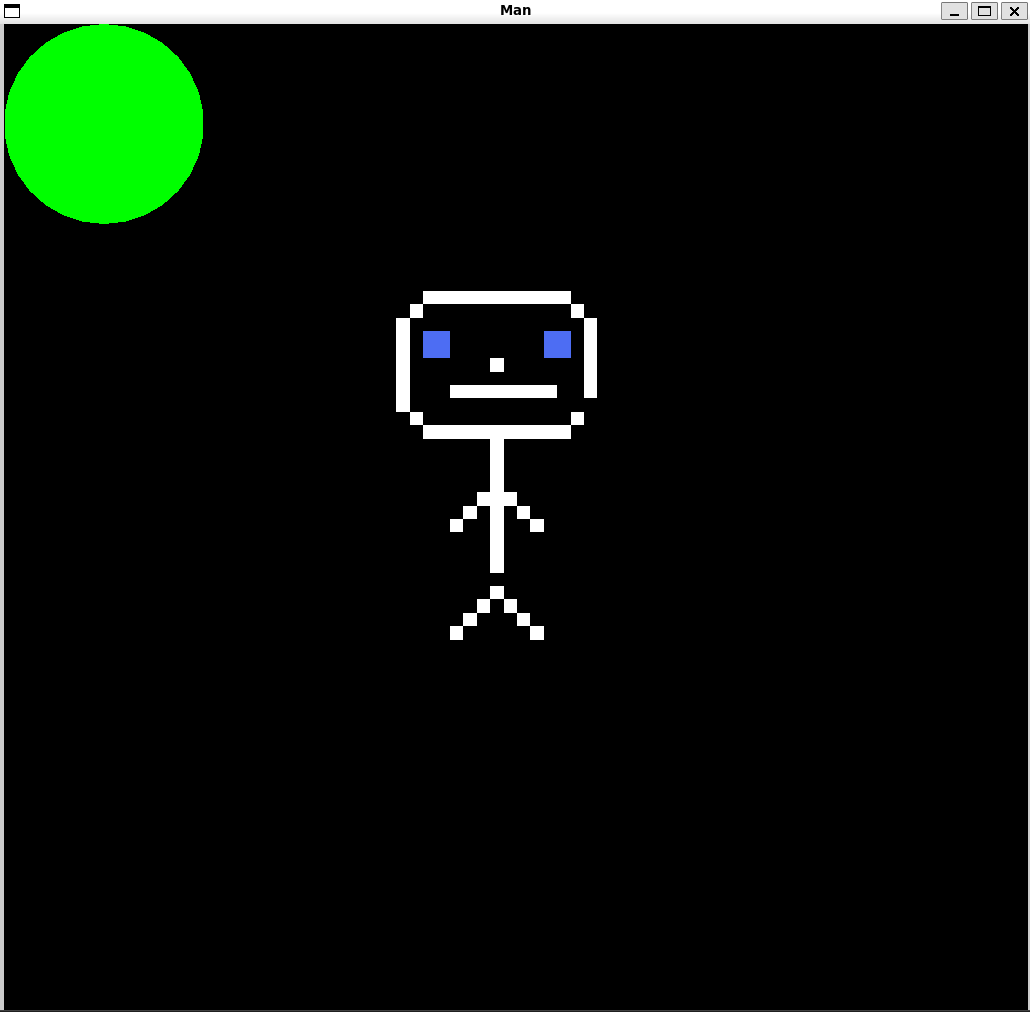
\includegraphics[width=0.8\textwidth]{"C:/Users/thoma/Downloads/Technical Papers/code pdfs/ps0/ps0_output.png"}
  \caption{ps0 program output}
  \label{fig:ps0_output}
\end{figure}

\section[5]{Issues and bugs}
\hfill\begin{minipage}{\dimexpr\textwidth-1cm}
No issues or bugs present. \newline
The program was fully functional within the given specification.
\end{minipage}

\section[6]{Source code for the project}


%ps0 pages 1-3

%\\\\\\\\\\\\\\\\\\\\\\\\\\\\\\\\\\\\\\\\\\\\\\\\\\\\\\\\\\\\\\\\\\\\\\\\\\\\\\\\\\\\\\\\\\\\\\\\\\\\\\\\\\\\\\\\\\\\\\\\\\\\\\\\\
\setcounter{section}{0}
\newpage
\section*{PS1 Linear Feedback Shift Register and Image Encoding}
\section[1]{Description of the assignment}
\hfill\begin{minipage}{\dimexpr\textwidth-1cm}
For part (a) of the assignment I implemented a 16 bit linear feedback shift register of class FibLFSR which generates a pseudo-random string of bits from a given seed. Using constant “tap” points at indices 15, 13, 12, and 10, bits are XOR’d together to generate a new input bit, which is then pushed back onto the register at index 0 which cycles out the bit at index 15. This process was used to generate a single bit using the step() function defined in line 18 of FibLFSR.cpp, as well as pseudo-random integers of size 0 – 2k by calling the generate(int k) function defined in line 31 of FibLFSR.cpp. To cleanse the input data for the constructor, exceptions were thrown if the seed string was not 16 bits in length, or if the seed string contained non-binary characters. \newline
I created two helper functions on lines 56 and 60 for the XOR of two bits a and b, and for the cleaning of a string to binary characters. Additionally I added const getters on lines 42 and 45, but no setters as end-users do not need to alter the internal state of the FibLFSR model. The output operator was also overloaded at line 50 to easily output the internal state of the FibLFSR object to the end user’s ostream. \newline
\newline
For part (b) of the assignment I encrypted a reference image using my FibLFSR from part (a). I created two RenderWindow objects “Base Image” and “Encrypted Image”. In my example program I encoded the Mona Lisa using my LFSR, then decrypted the image back into the Mona Lisa using the same seed for the LFSR. The encryption process occurred in the transform() function with an image by reference and pointer to a FibLFSR object as parameters.
\end{minipage}

\section[2]{Key algorithms, Data structures, or OO designs}
\hfill\begin{minipage}{\dimexpr\textwidth-1cm}
For part (a) the data structure used for bit storage was a bitset from the bitset library. This structure allowed for an easy conversion from string to bitset using the constructor bitset(string). This structure also allows for easy bit-shifting when the step() method is called, limiting unnecessary function calls and maximizing speed. \newline
\newline
For part (b) the key algorithm was the transform() function. This algorithm took each pixel of the given image and XOR’d the rgb values with a newly generated 8-bit integer from the given FibLFSR. The decryption algorithm used this same transform() function with an identically seeded LFSR which generated the same 8-bit integers which inverted the rgb values of the same pixels in order of encryption.
\end{minipage}

\section[3]{What I learned from the project}
\hfill\begin{minipage}{\dimexpr\textwidth-1cm}
For part (a) I learned the importance of choosing the correct data structure for the project at hand. I first attempted to use a std::string as my state storage method, but this object proved cumbersome when shifting bits. I tested a doubly-linked-list approach but this gave trouble when accessing tap-points. After doing some research I found the bitset library had the necessary built-in methods I was searching for, making the implementation of my own methods easy and intuitive. \newline
\newline
For part (b) I learned the importance of using sprite objects over texture objects due to their decreased system impact. Additionally I learned how to effectively gather command-line arguments for program execution, including file names and binary strings. Finally, I learned about rgb information in color objects, allowing for the augmentation and extraction of exact color values.
\end{minipage}

\section[4]{Screenshot of program output}
\begin{figure}[H]
  \centering
  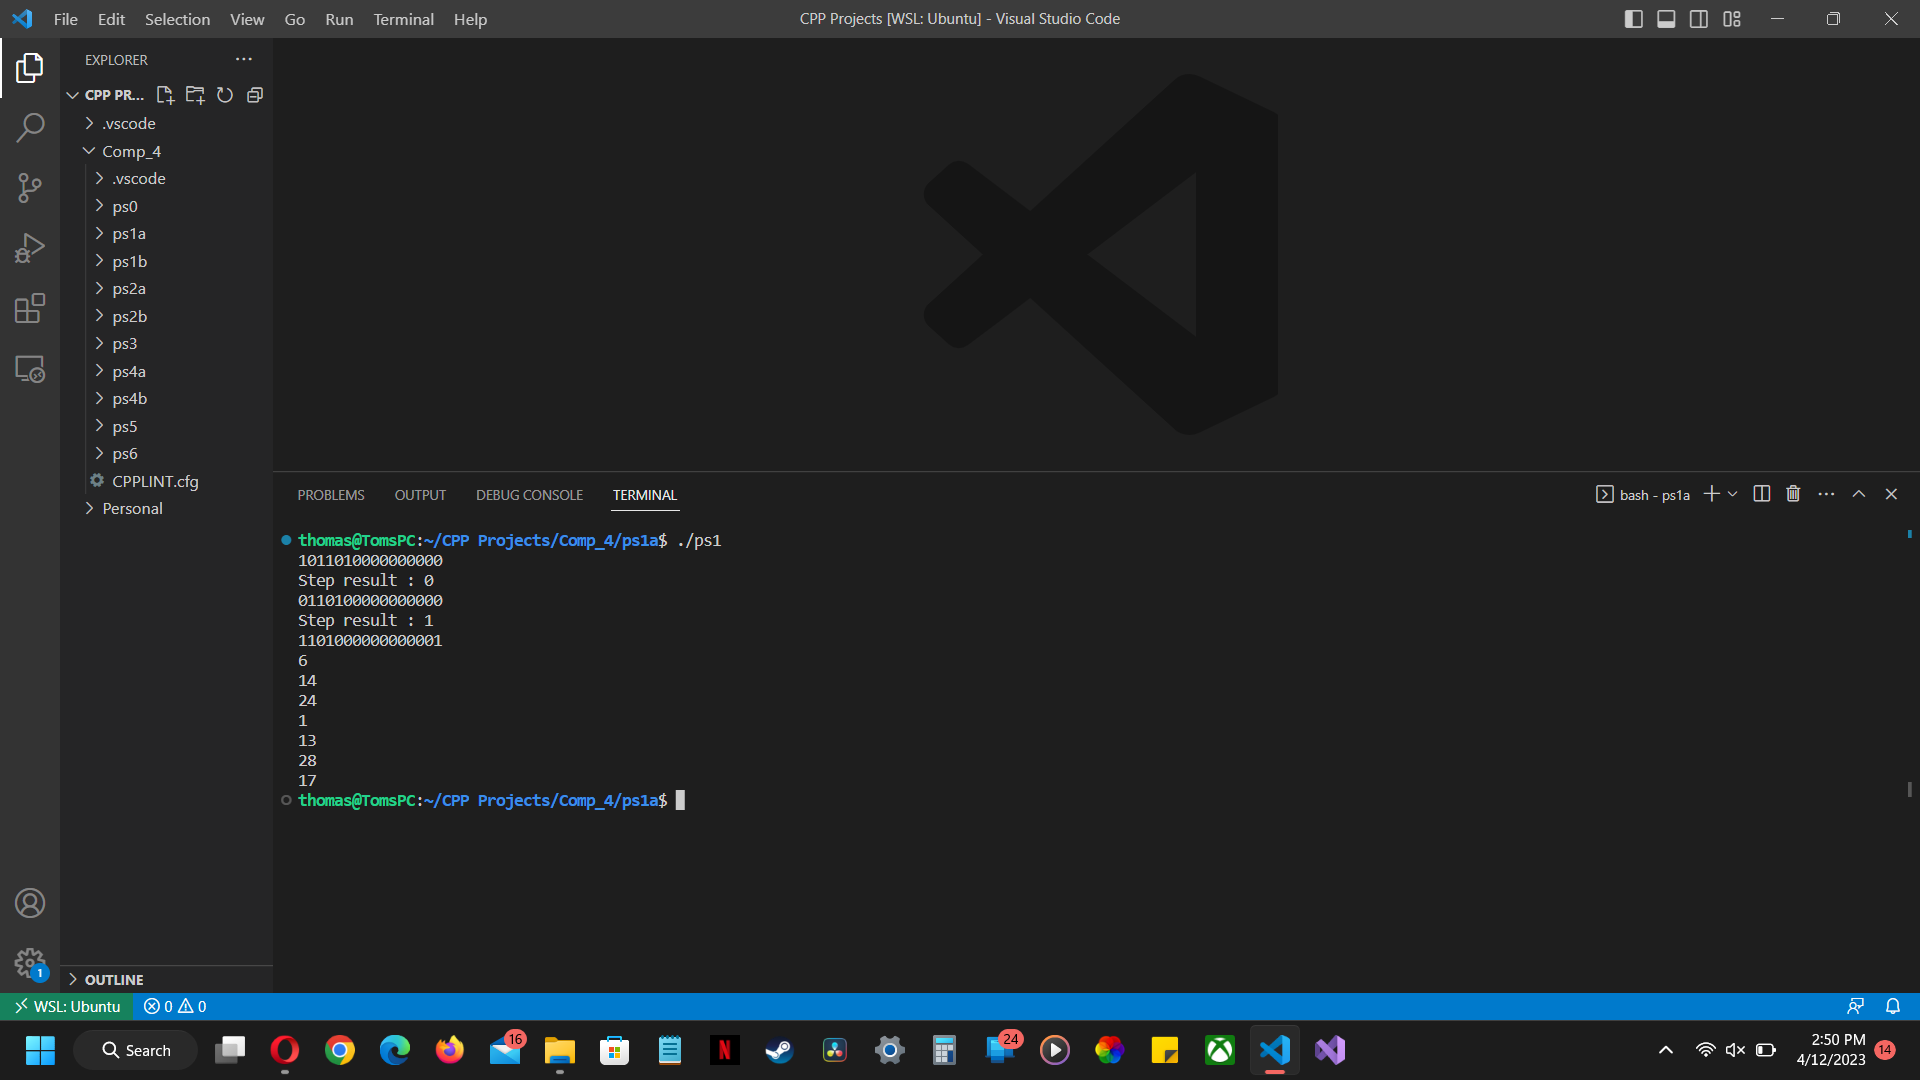
\includegraphics[width=0.9\textwidth]{"C:/Users/thoma/Downloads/Technical Papers/code pdfs/ps1/ps1a_output.png"}
  \caption{ps1a program output}
  \label{fig:ps1a_output}
\end{figure}
\begin{figure}[H]
  \centering
  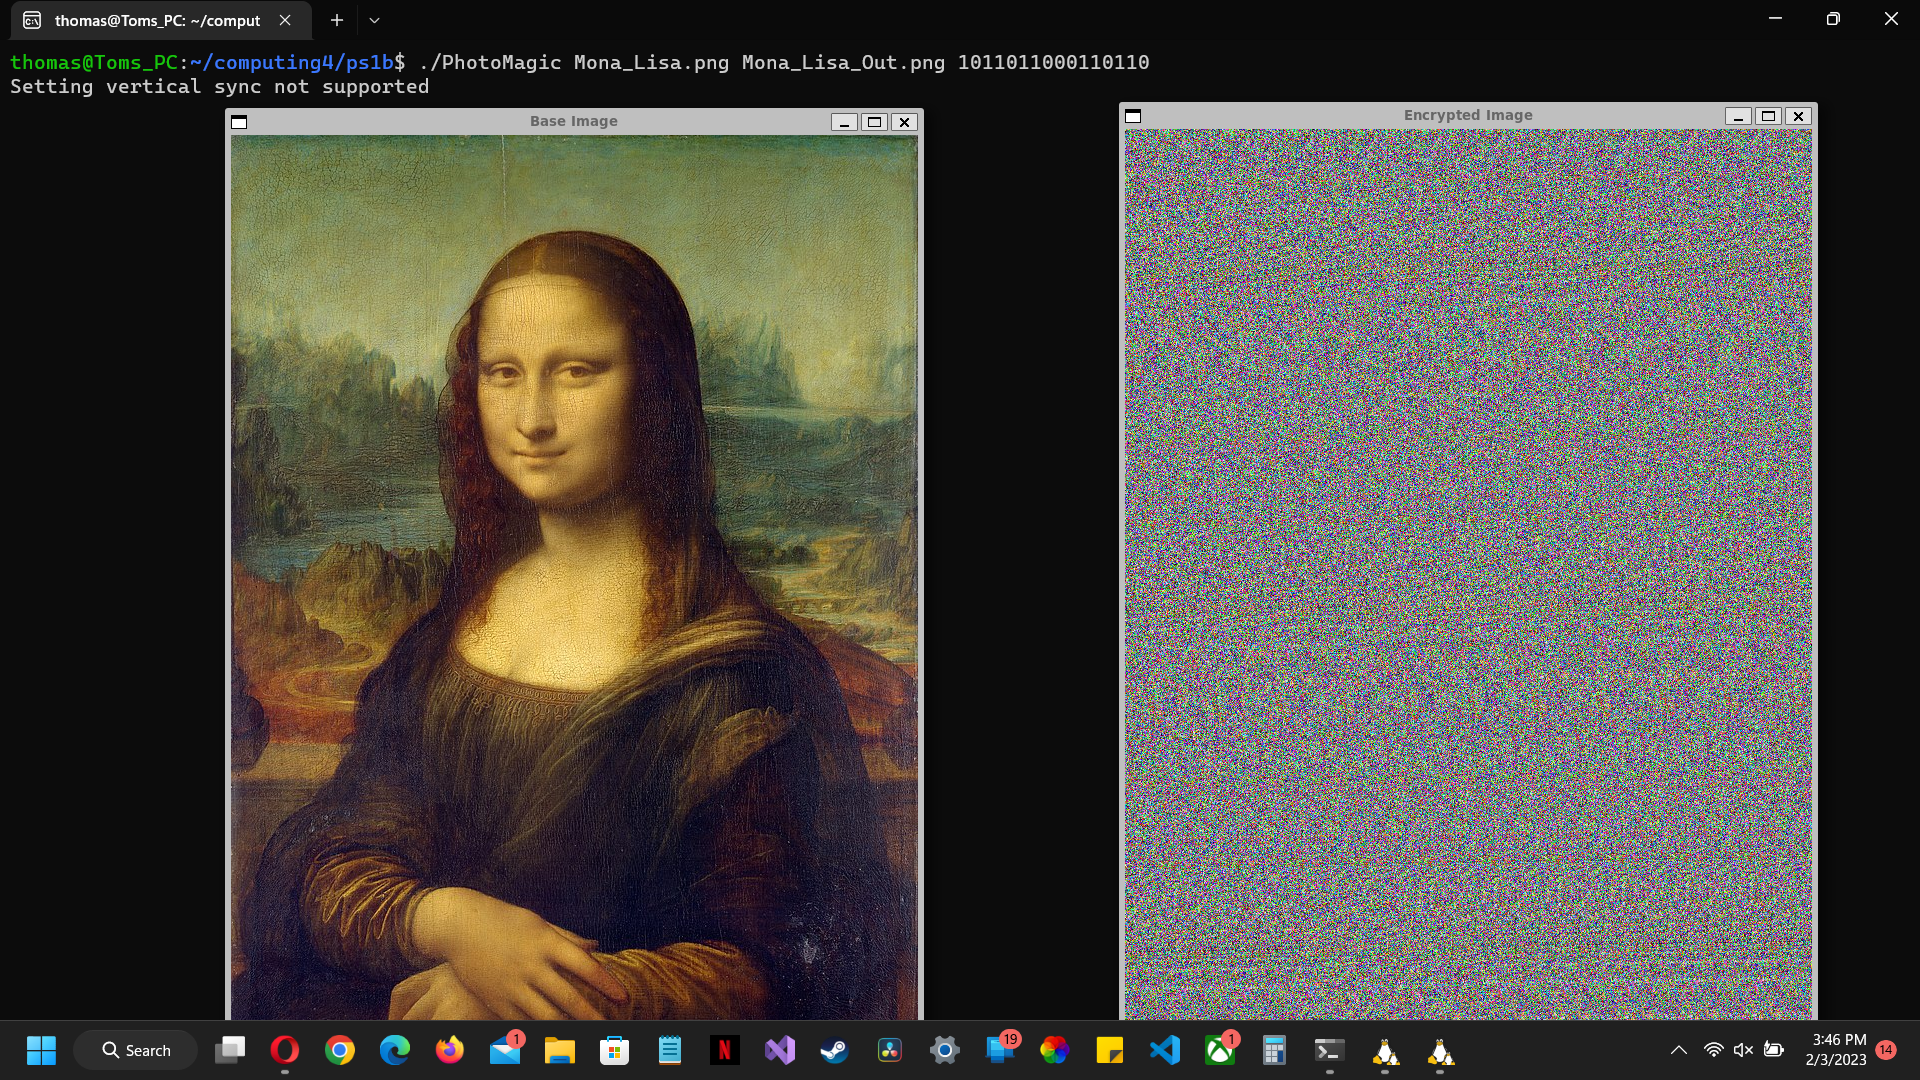
\includegraphics[width=0.8\textwidth]{"C:/Users/thoma/Downloads/Technical Papers/code pdfs/ps1/ps1b_Encryption.png"}
  \caption{ps1b encryption output}
  \label{fig:ps1b_Eoutput}
\end{figure}
\begin{figure}[H]
  \centering
  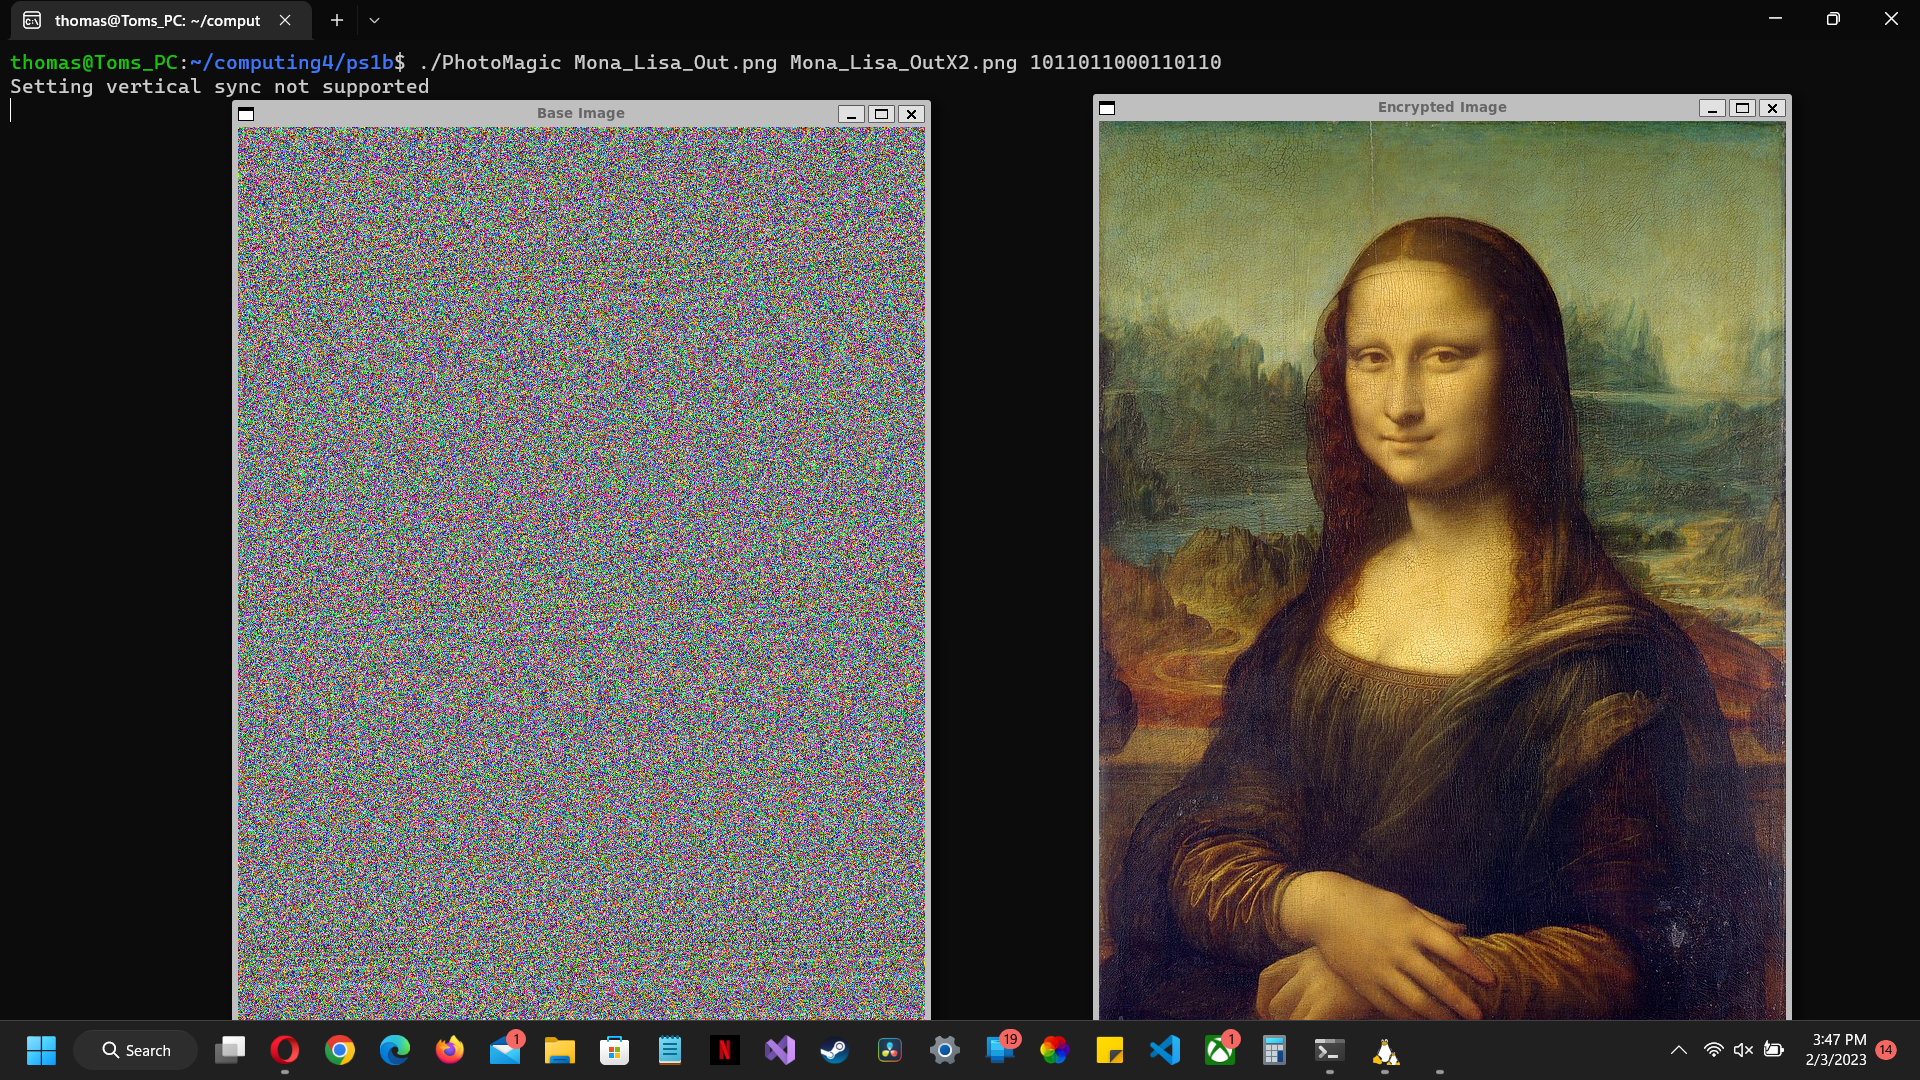
\includegraphics[width=0.8\textwidth]{"C:/Users/thoma/Downloads/Technical Papers/code pdfs/ps1/ps1b_Decryption.png"}
  \caption{ps1b decryption output}
  \label{fig:ps1b_Doutput}
\end{figure}

\section[5]{Issues and bugs}
\hfill\begin{minipage}{\dimexpr\textwidth-1cm}
No issues or bugs present. \newline
The program was fully functional within the given specification.
\end{minipage}

\section[6]{Source code for the project}

%ps1 pages 4-6

%\\\\\\\\\\\\\\\\\\\\\\\\\\\\\\\\\\\\\\\\\\\\\\\\\\\\\\\\\\\\\\\\\\\\\\\\\\\\\\\\\\\\\\\\\\\\\\\\\\\\\\\\\\\\\\\\\\\\\\\\\\\\\\\\\
\setcounter{section}{0}
\newpage
\section*{PS2 Sokoban}
\section[1]{Description of the assignment}
\hfill\begin{minipage}{\dimexpr\textwidth-1cm}
For part (a) of the assignment I created a Sokoban UI that inherited the virtual draw() function from the sf::Drawable class. This Sokoban class took in a file name from the command line, then opened the file and extracted the game state into the Game object using the overloaded extraction operator.
\begin{description}
\item In these .lvl files, the following symbols are used:
\item \textbf{@} The initial position of the player. Each level contains exactly one @.
\item \textbf{.} An empty space, which the player can move through.
\item \textbf{\#} A wall, which blocks movement.
\item \textbf{A} A box, which can be pushed by the player.
\item \textbf{a} A storage location, where the player is trying to push a box.
\item \textbf{1} A box that is already in a storage location.
\end{description}
A window titled “sokoban” was created in the exact dimensions of the level detailed in the file (64Wx64H). Each tile was 64 pixels on each side, making tileability easy. The window depicted tiles in their corresponding locations from the .lvl file. Additionally, a gameplay clock was included in the upper left corner of the window that displayed the elapsed time. I provided getters for internal variables, as well as a custom getGameState() function which printed the internal representation of the gameState to the terminal, which I used for debugging the value constructor and extraction operator. \newline
\newline
For part (b) of the assignment I implemented movement and gameplay mechanics. Using the (W,A,S,D) keys or (UP, DOWN, LEFT, RIGHT) keys, the end user could move the “janitor” character around the level through empty tiles, could push boxes onto other empty tiles, and could push boxes onto storage locations where they would change texture, indicating a successful storage. The player could not walk through walls, push boxes into walls, or push boxes into other boxes. The player could also walk through the empty storage locations. When all storage locations are filled with boxes, a win screen was presented to the user along with a win fanfare. This win screen presented the user’s completion time. The player had access to additional commands: (R) to restart the game, (Z) to undo turns, and (X) to close the window.
\end{minipage}


\section[2]{Key algorithms, Data structures, or OO designs}
\hfill\begin{minipage}{\dimexpr\textwidth-1cm}
In part (a) the data structure I used was a 2D vector of chars. This vector was resized to WxH from the input file, then filled with the corresponding symbols. This 2D vector stored the game in row-major order, since the IDE reads in a file in row-major order. The second component was the algorithm in the draw() function override, where a switch statement triggered the drawing of the appropriately textured sprite. \newline
In part (b) the primary data structure I used was a 3D vector of chars. This variable “allGameStates” stored the 2D matrix of game states as in part (a), but a third vector was added to include the undo function. Alongside a “turn” variable, every movement of the player incremented the turn variable and created a new game state matrix, pushing it back onto the 3D vector. If the player attempted to undo an action with command (Z), the game state would revert to the previous matrix at turn -1 for each undo action requested. Then as the player resumed normal movement, the matrix would overwrite with the new game states. \newline
In conjunction with the 3D vector and the turn variable, a new vector of type Direction was created labeled “face”. This vector was indexed using “turn” and corresponded to the direction the player character was facing. As the player moved in a particular Direction, the texture of the character was updated accordingly. As the player performed undo commands, the character direction would correspond to the movement actions of previous turns.
\end{minipage}

\section[3]{What I learned from the project}
\hfill\begin{minipage}{\dimexpr\textwidth-1cm}
For part (a) I learned about the power of nested data structures. Rather than allocating one large block of memory and doing coordinate arithmetic to locate my indices, I could use easily manageable structures with sensible indexing notation. I made frequent use of the double square-bracket operator (gameState[h][w]). This notation corresponded with my mental interpretation of the game board which sped up my coding and reduced out\_of\_bounds errors from the vectors. I was also reminded of the importance and power of defining global variables. In the case of ps2a, I defined a TILE\_SIZE int of size 64, indicating the pixel dimensions of my tiles. \newline
For part (b) I familiarized myself with companion data structures, using the same indexing element “turn” to access concurrent states across different objects. I had initial trouble combining player directionality and undo commands. Using a vector of directions allowed me to store the history of player movement at each “turn” and correspond it to the player character at any “turn”, regardless of direction of movement through the 3rd game state vector. \newline
Additionally, I familiarized myself with offloading work to private helper functions. These functions include noObstructions() at line 106, canPushBox() at line 172, and pushBox() at line 206 of Sokoban.cpp. I deferred complex calculations, bounds-detection, and movements outside of function movePlayer() at line 32.
\end{minipage}

\section[4]{Screenshot of program output}
\begin{figure}[H]
  \centering
  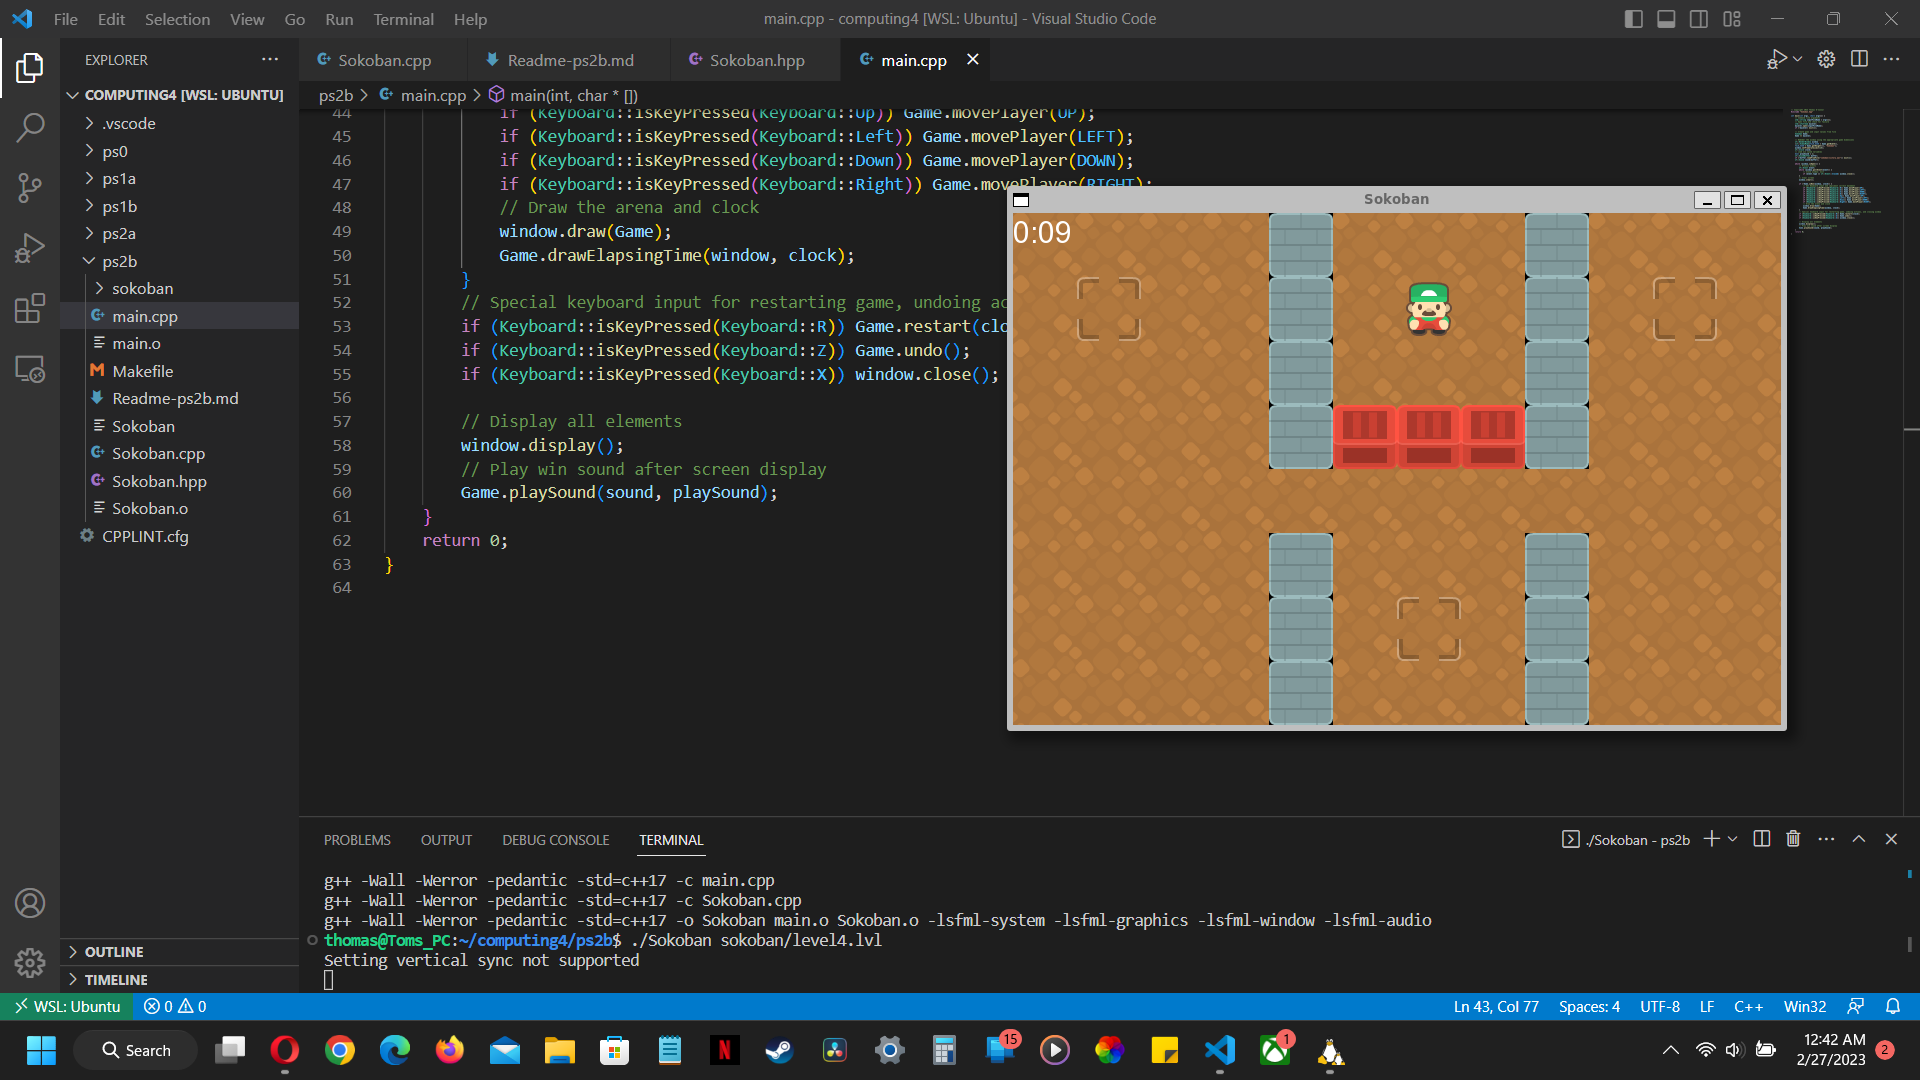
\includegraphics[width=0.9\textwidth]{"C:/Users/thoma/Downloads/Technical Papers/code pdfs/ps2/ps2b_output.png"}
  \caption{ps2b game output}
  \label{fig:ps2b_output}
\end{figure}

\section[5]{Issues and bugs}
\hfill\begin{minipage}{\dimexpr\textwidth-1cm}
\begin{itemize}
\item The Janitor was unable to push stored boxes out of storage areas.
\item The stored boxes updated texture from red to blue and behaved as walls.
\item Occasionally, textures flickered.
\end{itemize}
Otherwise, the program was functional within the given specification.
\end{minipage}

% bullet points

\section[6]{Source code for the project}

% ps2 pages 7-9

%\\\\\\\\\\\\\\\\\\\\\\\\\\\\\\\\\\\\\\\\\\\\\\\\\\\\\\\\\\\\\\\\\\\\\\\\\\\\\\\\\\\\\\\\\\\\\\\\\\\\\\\\\\\\\\\\\\\\\\\\\\\\\\\\\
\setcounter{section}{0}
\newpage
\section*{PS3 Pythagorean Tree }
\section[1]{Description of the assignment}
\hfill\begin{minipage}{\dimexpr\textwidth-1cm}
For this assignment I created a PTree class that recursively drew a Pythagorean tree of pixel size L and depth of N. A Pythagoras tree is a plane fractal constructed from squares whose points in connection to other squares enclose a right triangle.
\end{minipage}

\section[2]{Key algorithms, Data structures, or OO designs}
\hfill\begin{minipage}{\dimexpr\textwidth-1cm}
The key algorithm used to draw the tree was the PTree function defined at line 26 of PTree.cpp. The algorithm processes the points where new squares should be drawn. Given the angle of the parent square, the angles of the child squares are calculated and rotated accordingly. Based off of the two new child squares, 4 sets of points are calculated: the left child set and right child set. The PTree function is then recursively called on the left and right sets of points until it has reached the maximum depth N. Each depth is set to a different color.
\end{minipage}

\section[3]{What I learned from the project}
\hfill\begin{minipage}{\dimexpr\textwidth-1cm}
In this assignment I learned to delegate some of the work to an algorithm rather than static storage variables in my class type. The only variables of concern for the drawing of the PTree are the depth N and the length L. All other elements of the tree can be calculated from these two variables: no internal storage structure needed.
\end{minipage}

\section[4]{Screenshot of program output}
\begin{figure}[H]
  \centering
  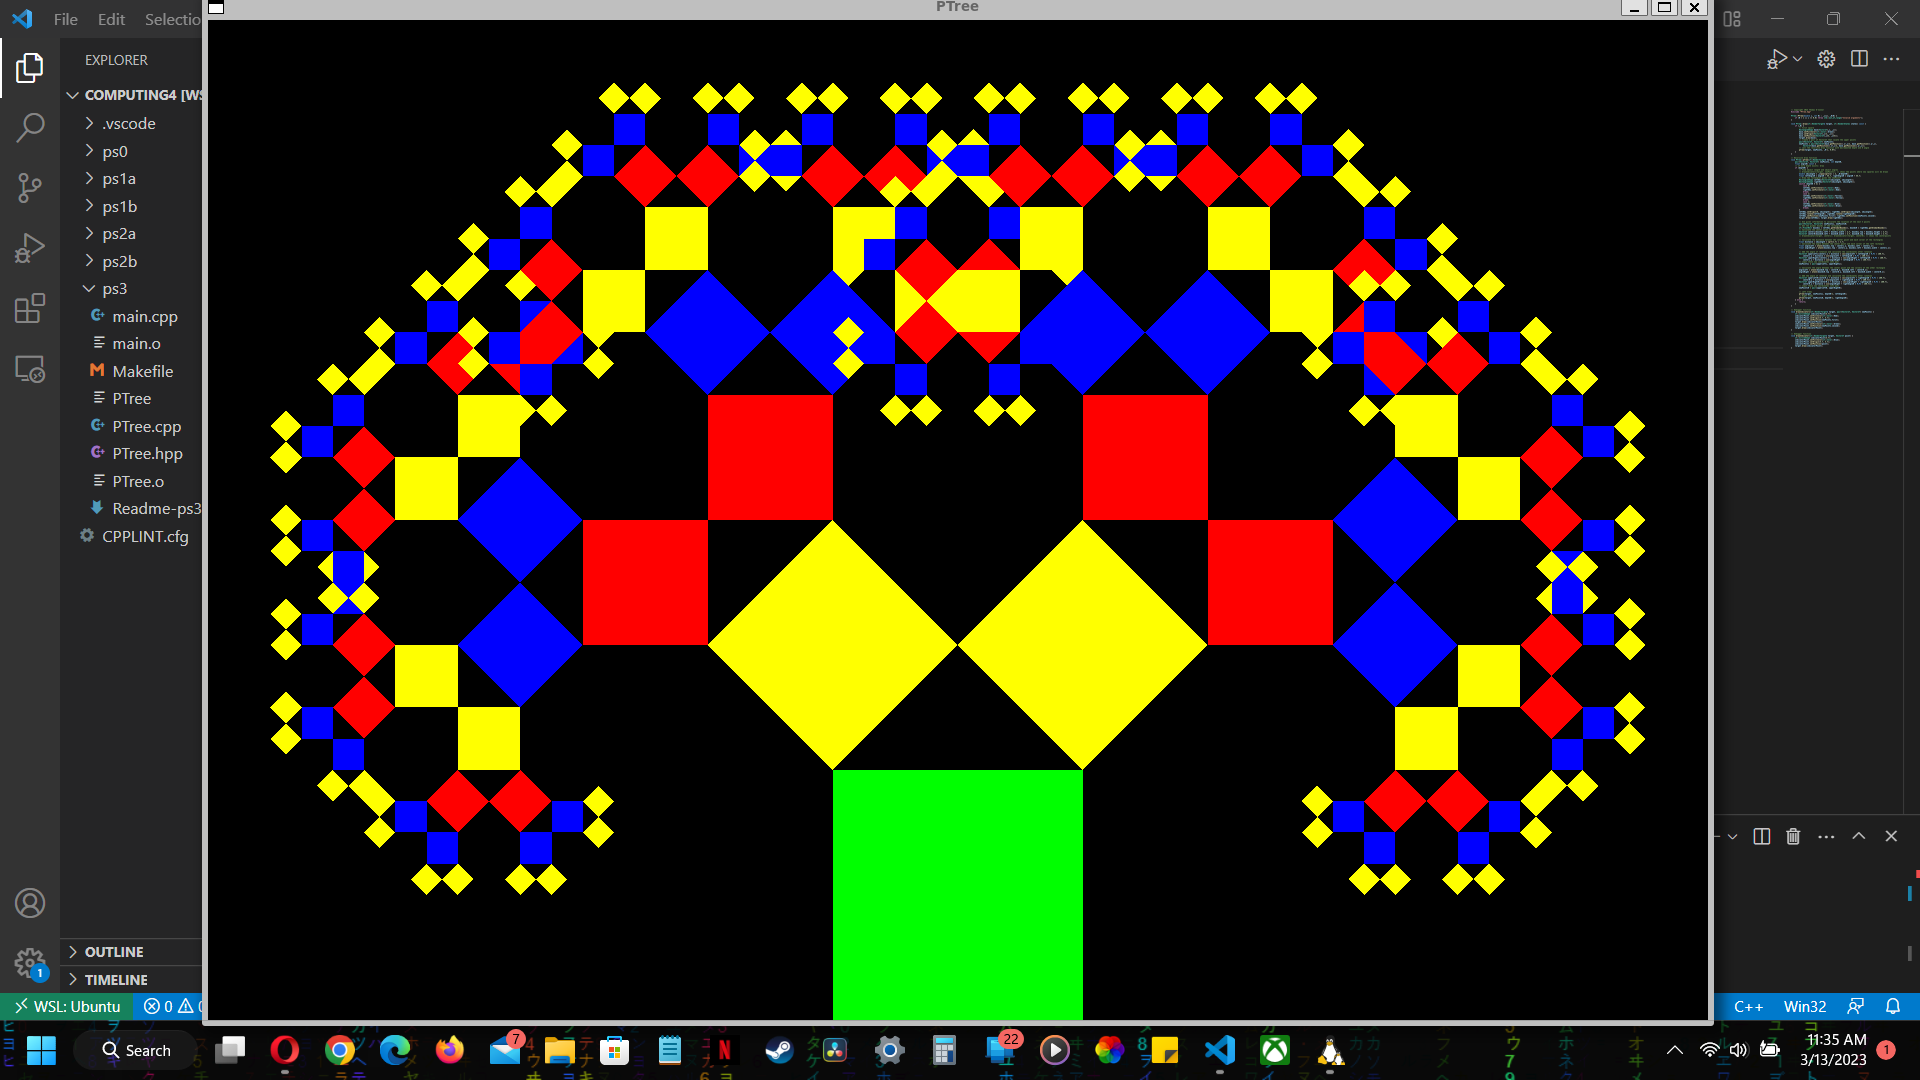
\includegraphics[width=0.9\textwidth]{"C:/Users/thoma/Downloads/Technical Papers/code pdfs/ps3/ps3_output.png"}
  \caption{ps3 tree output}
  \label{fig:ps3_output}
\end{figure}

\section[5]{Issues and bugs}
\hfill\begin{minipage}{\dimexpr\textwidth-1cm}
No issues or bugs present. \newline
The program was fully functional within the given specification.
\end{minipage}

\section[6]{Source code for the project}

% ps3 pages 10-12 TODO

%\\\\\\\\\\\\\\\\\\\\\\\\\\\\\\\\\\\\\\\\\\\\\\\\\\\\\\\\\\\\\\\\\\\\\\\\\\\\\\\\\\\\\\\\\\\\\\\\\\\\\\\\\\\\\\\\\\\\\\\\\\\\\\\\\
\setcounter{section}{0}
\newpage
\section*{PS4 Checkers}
\section[1]{Description of the assignment}
\hfill\begin{minipage}{\dimexpr\textwidth-1cm}
For part (a) of the assignment I created a Checkers UI that inherited the virtual draw() function from the sf::Drawable class. This Checkers class used an initializeBase() method defined at line 135 of Checkers.cpp to set the board and pieces to the default opening game configuration: 12 black pieces spread evenly on every black tile in the first three rows, and 12 red pieces spread evenly on every black tile over the last three rows. I defined two global variables: TILE\_SIZE of size 64 for the pixel size of the tiles, and BOARD\_DIMENSIONS of size 8 for the 8x8 dimensions of the game board. For extra credit I added an additional game border using a wood texture 32 pixels in depth. In part (a) I was also tasked with the selection of game pieces based on player turns. I created a mouseInGameBounds() helper function which determined if a mouse click was within the bounds of the game board including this new border texture. Using this helper function my selectPiece() method checked for the selection of a valid game piece by referencing the game data structure, the current player turn, and the number of non-selected pieces on the game board. Additionally I created a temporary switchTurn() method which artificially toggled the players’ turns. The default first player was black, and when the end user pressed (T) this was toggled to red. Based on the current player’s turn the end user could only select pieces of the current player. Clicking elsewhere would de-select a piece. At line 119 of Checkers.cpp I added another extra credit element: an indicator for the end user displaying the current color’s turn. Using the arial font an uppercase R or B was displayed in the upper left hand corner of the game board. \newline
\newline
For part (b) of the assignment I implemented the Checkers gameplay mechanics. This included a movePiece() method, a visual move assist, and a win condition with fanfare. I defined a new global variable: BOARD\_OFFSET of size 32 representing the game border. To move selected pieces I implemented a movePiece() method defined at line 88 of Checkers.cpp. This function manually checks the diagonal directions for moves and jumps, and completes the action if the mouse click was at one of the available end locations. At the end of this movement the finishLine() method is called which checks for the automatic crowning of pawns at the opponent’s end of the board. In addition to the movePiece() method, the visualMoveAssist() method defined at line 292 uses the same diagonal direction checking and displays a star diagonal to the selected piece on moveable tiles using the drawStar() helper function. The win fanfare was triggered by the isWon() method which checked for any remaining pieces or selected pieces, or triggered a win if no pieces could move. This then triggered an execution of code in main.cpp at line 43 which played a win sound, displayed the color of the winning team in text, and disabled player movement. Afterwards or during the game, the end user could press (X) to close the window or (R) to restart the game. The restart function simply called initializeBase() on the game object and reset the win condition Boolean variable.
\end{minipage}

\section[2]{Key algorithms, Data structures, or OO designs}
\hfill\begin{minipage}{\dimexpr\textwidth-1cm}
In part (a) the data structure I used was a 2D vector of characters named currentGameState.
\begin{description}
\item The following symbols were used in the 2D game state vector:
\item \textbf{.} A red background tile. Movement here is invalid.
\item \textbf{p} A black background tile. These squares are “playable”.
\item \textbf{b} A black pawn.
\item \textbf{r} A red pawn.
\item \textbf{w} A selected pawn
\item \textbf{B} A black king.
\item \textbf{R} A red king.
\item \textbf{W} A selected king.
\end{description}
The initializeBase() method went through the 2D vector placing a red background tile on every other element, and based on the line placed either a black piece, red piece, or playable black background tile. \newline
My “controller” that translated global mouse coordinates to 2D vector coordinates was performed at line 26 of Checkers.cpp. This initializer converted mouseLocation coordinates to arenaLocation coordinates by removing the border size and dividing by the tile size for each dimension. This resulted in a coordinate valid within my currentGameState matrix. \newline
\newline
In part (b) I used the same 2D character matrix as in part (a), but added two internal Boolean variables: stillPlaying and setWinTrue. These Boolean variables were used for edge conditions around the win conditions. stillPlaying was used primarily in the movePiece() method to ensure the game did not end prematurely when a piece was selected, while setWinTrue was used to expedite the win condition when a the final selected piece could not move in any direction. These variables could have been offloaded to boundary checking functions but were easily implemented when stored in the internal game state. \newline
Throughout the implementation file I use the getter function getSelectedPawn() which uses two algorithms (std::find\_if and std::distance) alongside three lambda expressions to parse through my matrix and return the internal coordinates of the selected pawn. I could have completed this through traditional for loops but I wanted to challenge myself to use advanced coding algorithms to accomplish my end goals, even if it was just for practice. 
\end{minipage}

\section[3]{What I learned from the project}
\hfill\begin{minipage}{\dimexpr\textwidth-1cm}
In part (a) of the assignment I learned the consequences of complicating my interior data storage structure. I chose to implement the red tiles in the matrix even though they would always be invalid tiles, never read or overwritten after initialization. This helped with conceptualization and debugging of the game board, since the interior state matched the real-life representation of the board. When moving on to part (b) however, this would result in complications. When performing checks on adjacent playable tiles I would always have to account for the 1x1 offset created by the red background tiles in all directions. This meant for more complex calculations and issues with the visual move assist.\newline
\newline
Over the course of part (b) of the assignment I learned to keep my functions simple and straightforward. I should have offloaded some of the work in movePiece() and visualMoveAssist() to helper functions that check diagonal boundaries. Because I did not use helper functions here, these methods were hundreds of lines long despite checking the exact same boundaries. I could have subdivided these checks in a variety of ways, but the brute force approach was what I chose to do despite of the obvious drawbacks.
\end{minipage}

\section[4]{Screenshot of program output}
\begin{figure}[H]
  \centering
  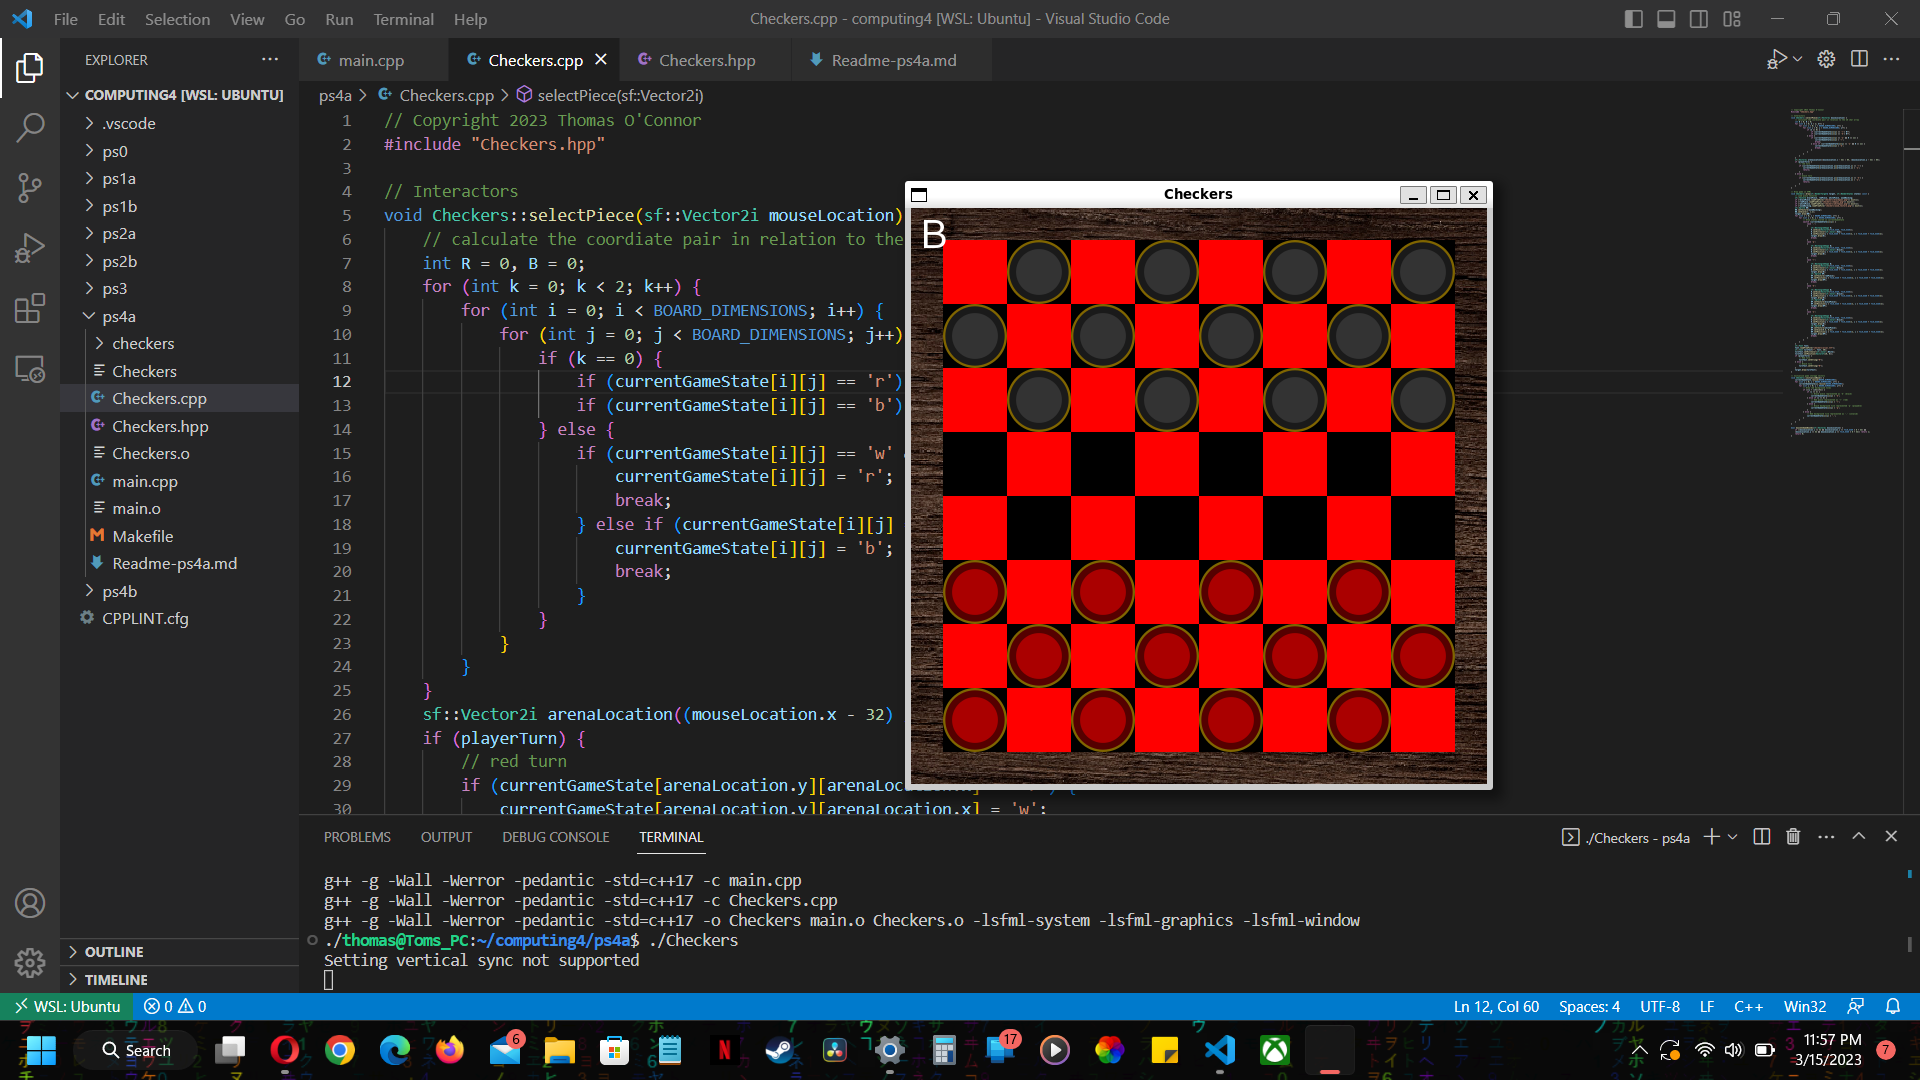
\includegraphics[width=0.9\textwidth]{"C:/Users/thoma/Downloads/Technical Papers/code pdfs/ps4/ps4_output.png"}
  \caption{ps4 game output}
  \label{fig:ps4_output}
\end{figure}

\section[5]{Issues and bugs}
\hfill\begin{minipage}{\dimexpr\textwidth-1cm}
\begin{description}
\item Pieces could not double jump.
\item Pieces that could jump were not required to jump.
\item If multiple pieces on the same team were all deadlocked, \newline \newline
win condition would never be met.
\item Occasionally, textures flickered.
\end{description}
Otherwise, the program was functional within the given specification.
\end{minipage}

\section[6]{Source code for the project}





%\\\\\\\\\\\\\\\\\\\\\\\\\\\\\\\\\\\\\\\\\\\\\\\\\\\\\\\\\\\\\\\\\\\\\\\\\\\\\\\\\\\\\\\\\\\\\\\\\\\\\\\\\\\\\\\\\\\\\\\\\\\\\\\\\
\setcounter{section}{0}
\newpage
\section*{PS5 DNA Alignment}
\section[1]{Description of the assignment}
\hfill\begin{minipage}{\dimexpr\textwidth-1cm}
In this assignment I created an EDistance class that computed the edit distance of two strings. Here the edit distance is the optimal alignment of the two strings. This optimal alignment is computed using a scoring system, where a gap in either string is a penalty of two, no gap but a misaligned letter is a penalty of one, and no gap and a matching letter is no penalty. The optimal edit distance has the lowest score, and is computed by dynamically allocating a matrix of integer values of size NxM, where N is the size of string one, plus one, and M is the size of string two, plus one. At the bottom right corner of the matrix is a score of zero. Here the strings “meet” when they are aligned. Going directly up or directly left from the bottom corner, the consecutive values increase by two, as this represents the penalty for a gap in either string. Beginning at the bottom right corner, the scoring algorithm is performed of all values remaining in the NxM matrix. This will be explained in the following section. After the matrix is filled in with scores, the optimal edit distance is found at (0, 0) of the matrix. \newline
\newline
In order to find the optimal alignment we must traverse this matrix with reference to the strings, using dashes as gaps in the final alignment. This algorithm will also be discussed in the following section. This can be used for any two strings of values, but its most useful application is the alignment of DNA, as shown in the test cases. My program computed the alignment for two strings of lengths 2,500, 5,000, 7,000, 10,000, 20,000, and 28,284, as well as multiple strings of lengths less than 100 characters. These strings were taken from stdin using the “<” redirect, and either output to the terminal in small cases, or output to a .txt document using the “>” redirect in large cases. 
\end{minipage}

\section[2]{Key algorithms, Data structures, or OO designs}
\hfill\begin{minipage}{\dimexpr\textwidth-1cm}
The two key algorithms used in this assignment were the scoring algorithm and the traversal algorithm. The scoring algorithm can be seen at line 27 of EDistance.cpp. The optDistance() method fills in the matrix using the following expression:

\[For\:each:\;0 <= i < M, 0 <= j < N\]
\[Matrix[i][j] = min ( matrix[i+1][j+1] + penalty(), matrix[i+1][j] + 2, matrix[i][j+1] + 2 )\]

This algorithm is executed from the bottom right of the matrix and compares values adjacent to and diagonal from the selected element. This is performed right to left, bottom to top. In the above expression, the penalty() method is the zero or one penalty from the character discrepancy check performed on the selected element. If the characters are different, a penalty of one is applied, else, zero. \newline
\newline
My implementation of the traversal algorithm can be seen in the alignment() method defined at line 40 of EDistance.cpp. This method starts at the top left of the scoring matrix and finds the optimal path to the bottom right. Unless at a boundary condition, the algorithm prioritizes diagonal checks, then subsequently checks for gaps in the alignment. In each case, there are a series of “if” statements that check to see if the scores at each position are equivalent to the currently selected element’s score, minus the penalty. This is either the static two or the zero/one based on the character discrepancy of the current element. The algorithm traces the matrix and only retrieves the optimal traversal, pushing the coordinates of each valid element back onto the optPath list in order. After the traversal is complete, beginning at line 70 of EDistance.cpp the list is parsed; and based on the diagonal or perpendicular movement the alignment is prepared using the reference strings’ characters and dashes to represent the gaps in alignment. This is assembled into a single contiguous string and returned by the method.
\end{minipage}

\section[3]{What I learned from the project}
\hfill\begin{minipage}{\dimexpr\textwidth-1cm}
In this assignment I learned the power of dynamic programming. Using a series of simple algorithms in combination with a fully adjustable dataset, my program could easily handle and calculate hundreds of millions of scores based off of multi-thousand character strings. This would have been effectively impossible to do by hand and without error, but my program was speedy and accurate every time. Moreover I learned about different approaches to the same problem: In this case DNA alignment. The spec outlined multiple tactics for approaching the problem, including recursive approaches, the Needleman-Wunsch method, and Hirschberg's algorithm, all with certain advantages and disadvantages. Based on my personal constraints and implementation I could adapt my method to prioritize storage space, cpu power, or processing time. \newline
\newline
An optional component of this assignment was to work with a partner; I chose to work alone on this assignment. This was because I wanted to challenge myself to conceptualize and implement my own interpretation of the problem. This may have taken more time overall, but I’m glad I tackled the problem independently because I now have a greater capacity to debug my code. For example: during this assignment I completed 90\% of the algorithm, but my results for the optimal alignment were off by two for all of the test cases. This problem stumped me for a while, and could have easily been remediated by a partner. By sitting with the problem and debugging my own code I found the issue not in my algorithm, but in my reading of the test case variables. If I had not worked alone on this assignment I wouldn’t have had that same struggle and intellectual payoff.
\end{minipage}

\section[4]{Screenshot of program output}
\begin{figure}[H]
  \centering
  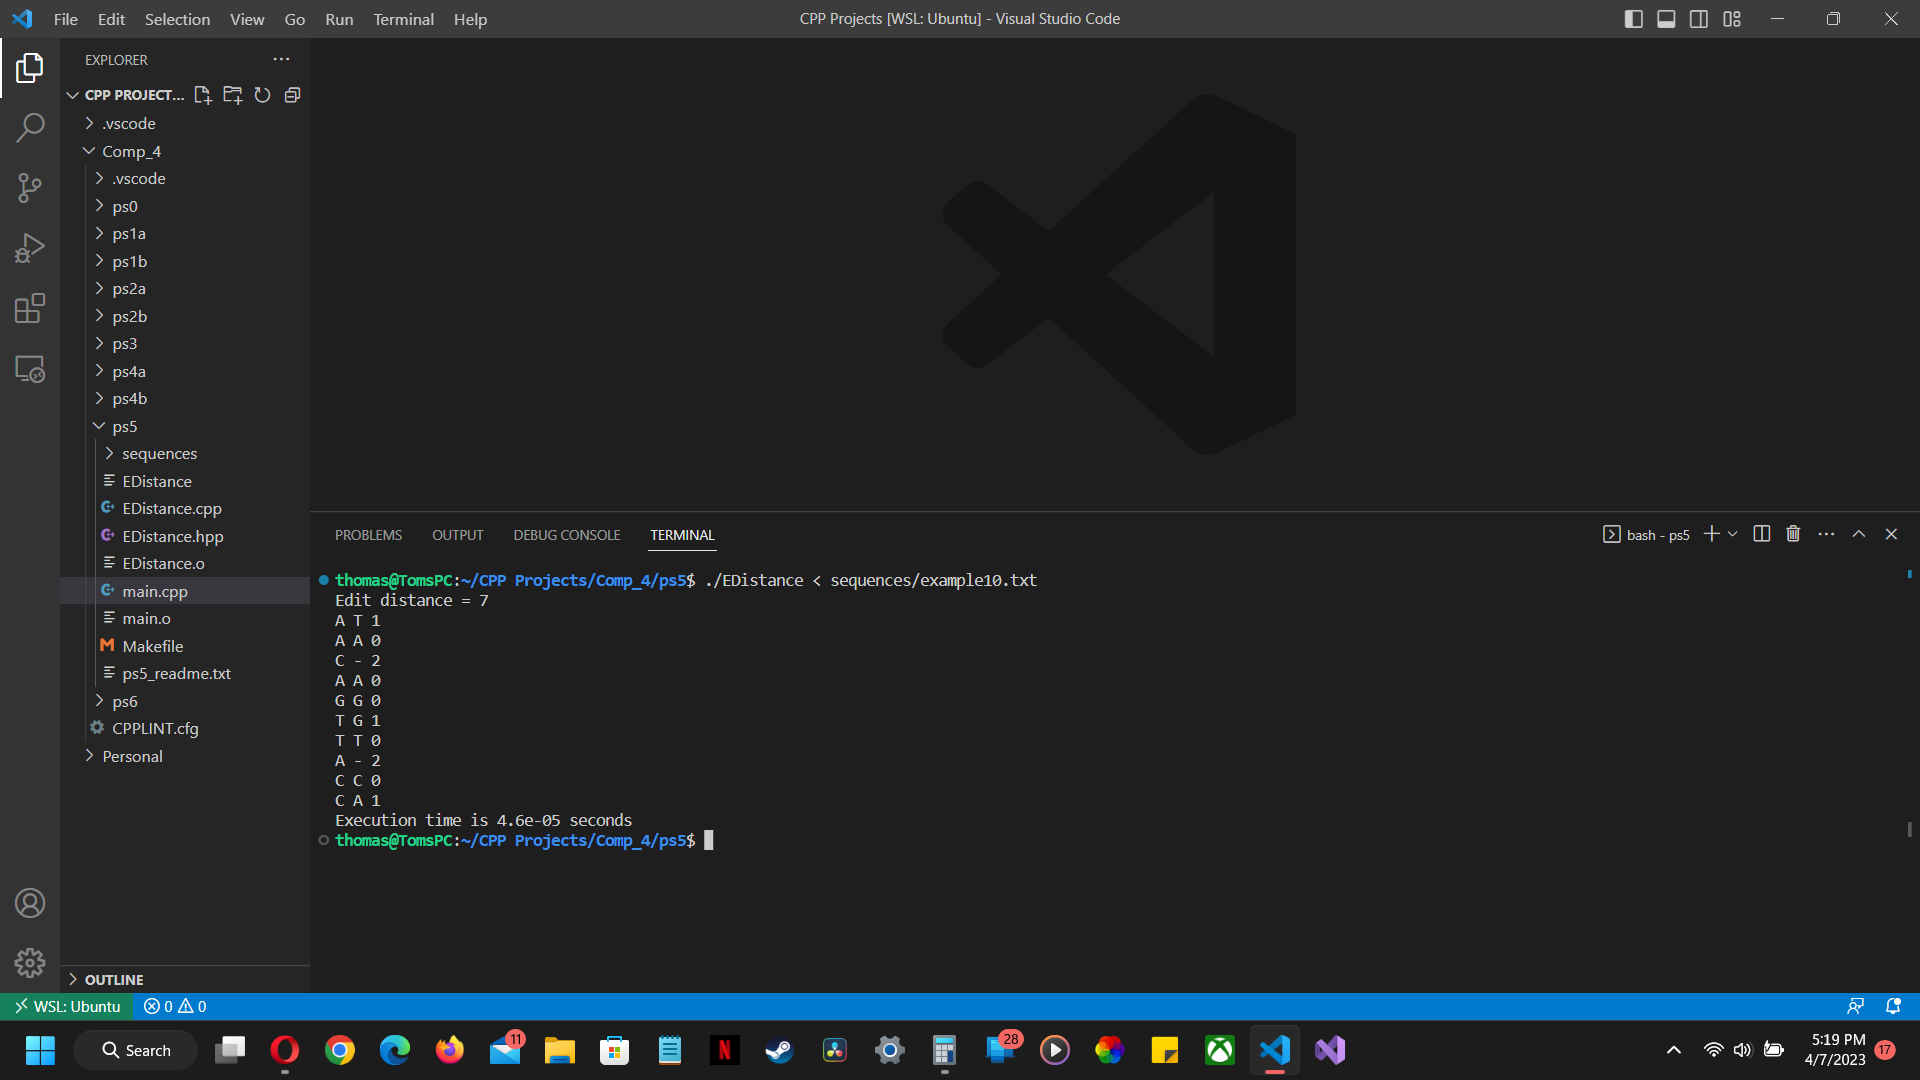
\includegraphics[width=0.9\textwidth]{"C:/Users/thoma/Downloads/Technical Papers/code pdfs/ps5/ps5_output.png"}
  \caption{ps5 terminal output}
  \label{fig:ps5_output}
\end{figure}

\section[5]{Issues and bugs}
\hfill\begin{minipage}{\dimexpr\textwidth-1cm}
No issues or bugs present. \newline
The program was fully functional within the given specification.
\end{minipage}

\section[6]{Source code for the project}





%\\\\\\\\\\\\\\\\\\\\\\\\\\\\\\\\\\\\\\\\\\\\\\\\\\\\\\\\\\\\\\\\\\\\\\\\\\\\\\\\\\\\\\\\\\\\\\\\\\\\\\\\\\\\\\\\\\\\\\\\\\\\\\\\\
\setcounter{section}{0}
\newpage
\section*{PS6 RandWriter}
\section[1]{Description of the assignment}
\hfill\begin{minipage}{\dimexpr\textwidth-1cm}
In this assignment I created a RandWriter class that writes random text based on a reference text. The main program takes in two integers: the first “K” which is the size of the subdivisions of the text, and “L” the length of the random text output. The object then read a reference text from std::cin, then developed “kgrams”, (N) strings of size K where N is the size of the reference text. Along with these kgrams, k+1grams were developed, which is every occurrence of the kgram followed by the subsequent character in the reference text. Using the kgrams and k+1grams, a probabilistic dictionary was developed for each potential string of size K (given that it appeared at least once in the text). To develop the random text output, the first K characters were used as the seeding value for the generate() method defined at line 78 of RandWriter.cpp. Each subsequent character was chosen from the probability dictionary of the current kgram which matches the relative distribution of characters that follow that kgram in the reference text. These characters were pushed back onto the output string until the string was of size L, then returned by the method. Text generated with a low K value (0-4) frequently produces unintelligible words, makes spelling mistakes, and includes inappropriate characters. Text generated with moderate K values (5-9) frequently produces intelligible words and phrases in the style of the reference text, although there are some evident discrepancies. Text generated with high K values (10 or greater) are very accurate with the reproduction of understandable text at the risk of copying the reference material word for word. This is because some kgrams of large size are unique in a text, which lead to the reproduction of multiple consecutive sentences or a whole paragraph ripped directly from the reference material.
\end{minipage}

\section[2]{Key algorithms, Data structures, or OO designs}
\hfill\begin{minipage}{\dimexpr\textwidth-1cm}
The key data structure used in this assignment was the Markov Model, which I chose to implement as an unordered map. This map contained the string kgrams as keys, and a pair of data: an int for the occurrences of the kgram, and a string for the probability dictionary of the k+1grams. The constructor for the object parsed through the reference text, and treated it as cyclical. For each occurrence of the kgram, the int at the kgram’s key in the model was incremented to show a new occurrence, and the following letter was appended to the dictionary string. After iterating through the entire reference text, the model would be full of every possible K sized string as well as the occurrences of that string and the following letters that followed it, stored in the form of one contiguous string. The interior state of this Markov Model could be output using the overloaded stream insertion operator. \newline
\newline
An algorithm that was used in the assignment was the kRand() method at line 57 of RandWriter.cpp. The kRand() method selected a random value from the probability dictionary at a given kgram by using a random\_device, a Mersenne Twister, and a uniform\_int\_distribution. The std::random\_device generated a pseudo-random integer which was used as the seed value for the Mersenne Twister. At line 68 of the implementation file a std::uniform\_int\_distribution was initialized with the bounds of the dictionary of the given kgram. A random character from the dictionary was then chosen and returned by the method using the Mersenne Twister as the seed for the uniform\_int\_distribution, where it would index a character within the bounds of the dictionary. \newline
\newline
One helper function that was used to complete the assignment was the cycleString() function defined at line 117 of RandWriter.cpp. This function modified a string in place by cycling the values to the left and pushing back a character item to the end of the string. This was used to parse through the reference text for all kgrams, and was used for the generate() method by converting k+1grams to new kgrams, which was then used to seed the new kRand() method. \newline
\newline
In order to deal with a potential K = 0, a global variable ORDERZERO was defined as the master reference key for the map, where the reference text itself was the probability dictionary. This meant that characters in the final text output were distributed randomly in the same proportions as they appeared in the reference text with no further context relative to kgrams.
\end{minipage}

\section[3]{What I learned from the project}
\hfill\begin{minipage}{\dimexpr\textwidth-1cm}
Looking back on the project I see that my internal Markov Model was inefficient. Rather than employing an unordered map of string keys with a pair of int and string as the data values, I should have simply used an unordered map of string keys and string data. This is because the int data in the pair is redundant. The frequency of the kgram in the reference text that the int is supposed to represent is also the size of the dictionary string. This did not effect the correctness of the text generation, but did impact the speed and efficiency of the model slightly by calling the increment operator once for every character in the reference text, as seen at line 21 of the implementation file.
\end{minipage}

\section[4]{Screenshot of program output}
\begin{figure}[H]
  \centering
  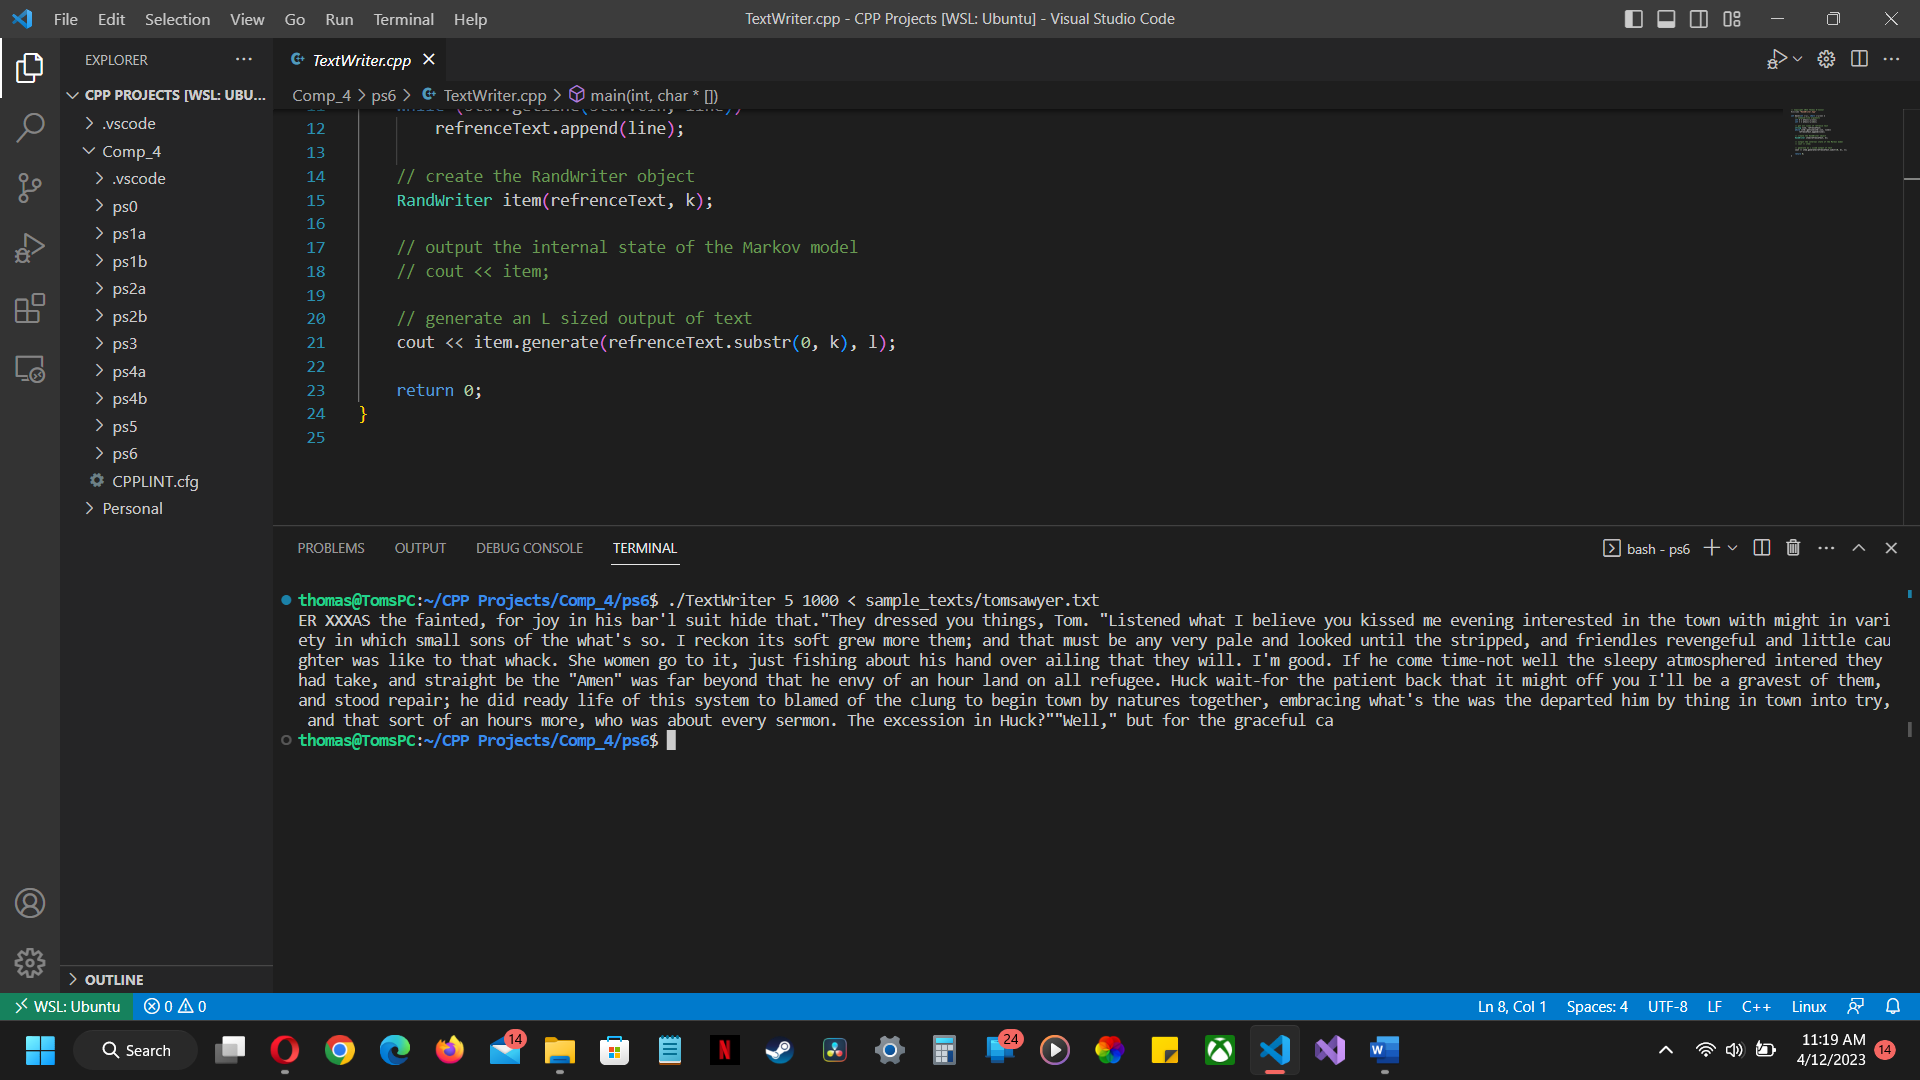
\includegraphics[width=0.9\textwidth]{"C:/Users/thoma/Downloads/Technical Papers/code pdfs/ps6/ps6_output.png"}
  \caption{ps6 terminal output}
  \label{fig:ps6_output}
\end{figure}

\section[5]{Issues and bugs}
\hfill\begin{minipage}{\dimexpr\textwidth-1cm}
No issues or bugs present. \newline
The program was fully functional within the given specification.
\end{minipage}

\section[6]{Source code for the project}





%\\\\\\\\\\\\\\\\\\\\\\\\\\\\\\\\\\\\\\\\\\\\\\\\\\\\\\\\\\\\\\\\\\\\\\\\\\\\\\\\\\\\\\\\\\\\\\\\\\\\\\\\\\\\\\\\\\\\\\\\\\\\\\\\\
\setcounter{section}{0}
\newpage
\section*{PS7 Kronos Log Parsing}
\section[1]{Description of the assignment}
\hfill\begin{minipage}{\dimexpr\textwidth-1cm}
In this assignment I created a LogParser class which accepted a std::ifstream input and the file path. This class then generated a report based on the log input using the generateRPT() method. The generate method logged the beginning, end, and failure of boot sequences for Kronos InTouch devices, assuming no nesting booting.
\end{minipage}

\section[2]{Key algorithms, Data structures, or OO designs}
\hfill\begin{minipage}{\dimexpr\textwidth-1cm}
The key algorithm used in my implementation was my generateRPT() method defined at line 4 of LogParser.cpp. This function parsed through Kronos .log files and generated a string which was output to a .log.rpt file in main.cpp at line 16. The algorithm used the syntax provided in the device5\_intouch.log\_BOOTONLY.rpt, noting the line and time of boot start, as well as the line and time of boot completion, and elapsed time, or the indication of an incomplete boot. The method performed this documentation across multiple attempted boot cycles. \newline
Another algorithm used can be found at lines 37 – 39 of the implementation file. These lines used ptime and time\_duration variables found in the boost::posix\_time library. The constructor of ptime automatically converts the date and time string to a valid posix\_time, then the time\_duration object retrieves the difference between the start and end times using the built-in subtraction operator and assignment operator. This time discrepancy is then reported in milliseconds as prescribed by the spec.

\end{minipage}

\section[3]{What I learned from the project}
\hfill\begin{minipage}{\dimexpr\textwidth-1cm}
In this assignment I learned about the effective use of regular expressions (regex). Rather than doing manual comparisons to predefined static strings, regexes allow you to catch expressions dynamically. If there is known variation in a program output, a regex may account for a variety of scenarios including unique number or name strings. In this assignment I used two regexes to catch the beginning and conclusion of the boot sequence.
\end{minipage}

\section[4]{Screenshot of program output}
\begin{figure}[H]
  \centering
  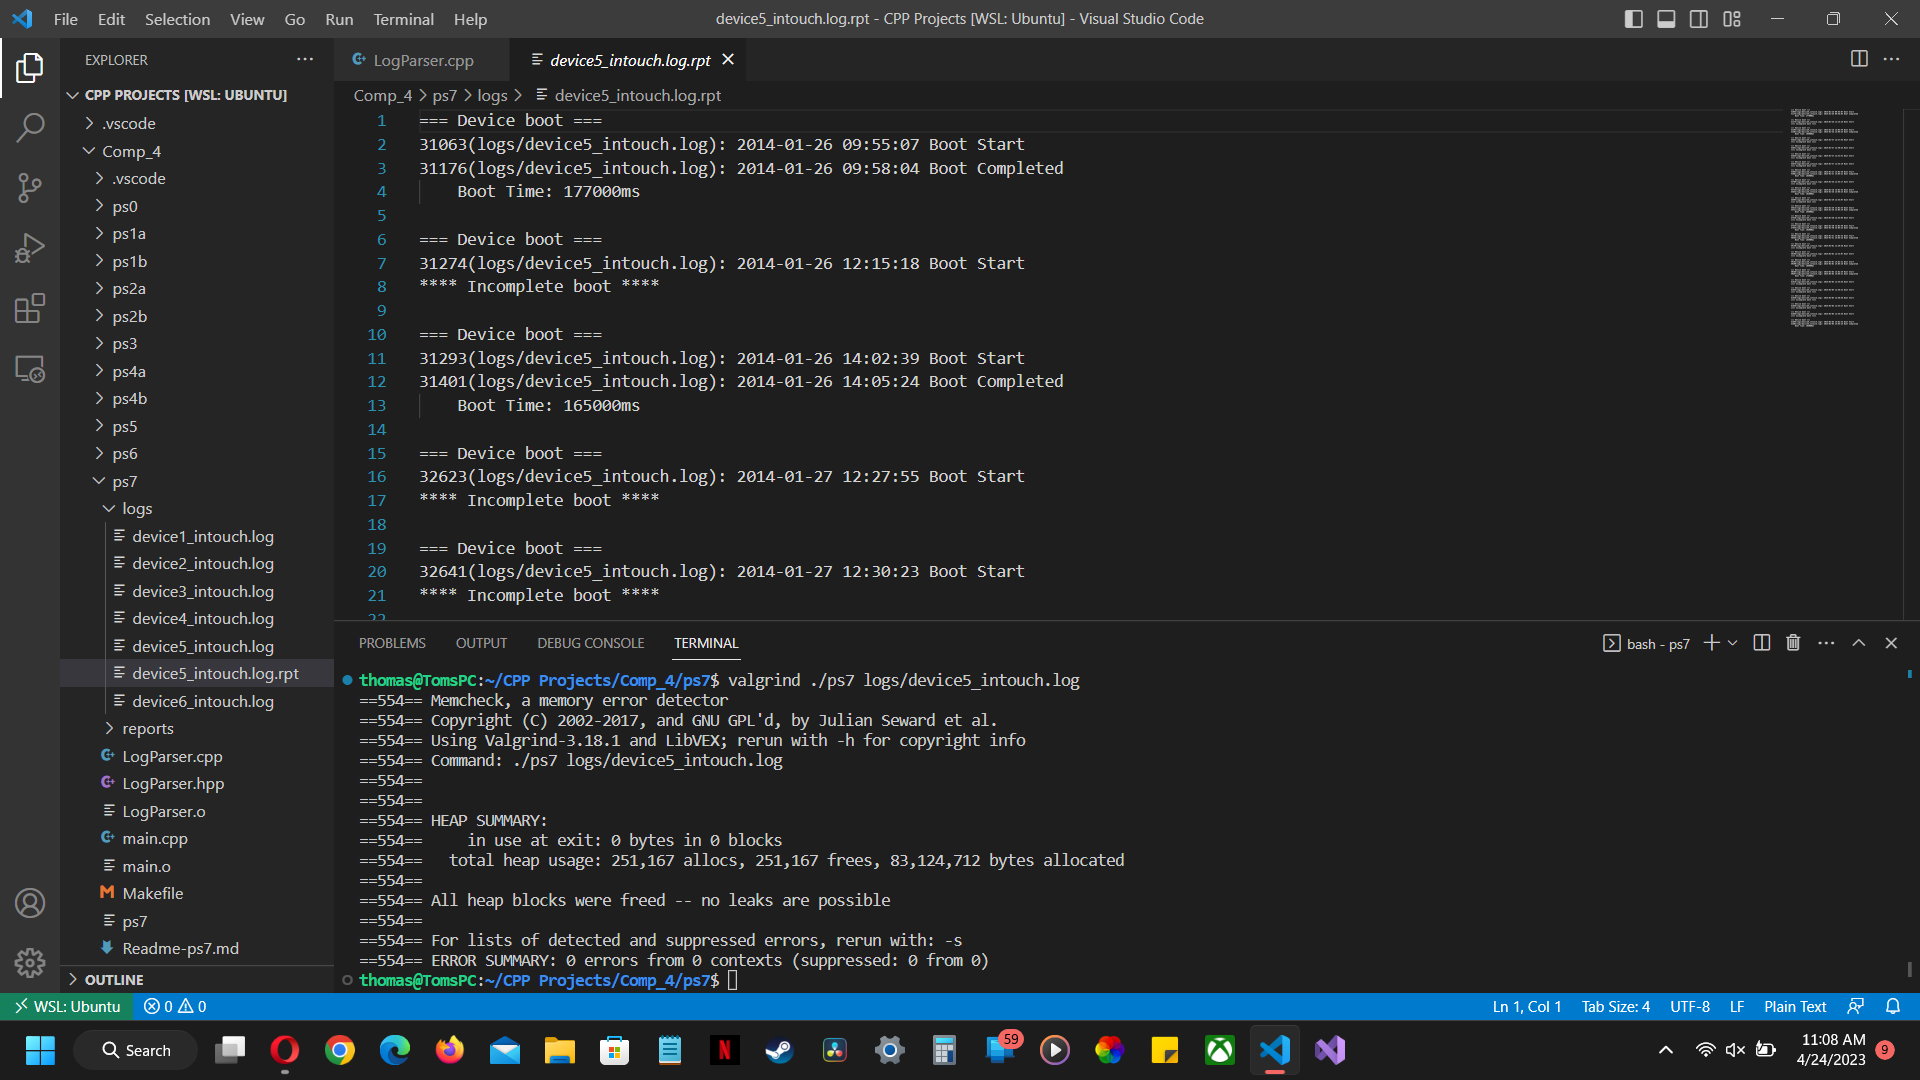
\includegraphics[width=0.9\textwidth]{"C:/Users/thoma/Downloads/Technical Papers/code pdfs/ps7/ps7_output.png"}
  \caption{ps7 .rpt output}
  \label{fig:ps7_output}
\end{figure}

\section[5]{Issues and bugs}
\hfill\begin{minipage}{\dimexpr\textwidth-1cm}
For all given logs, the provided implementation works. \newline
If another log file contains a different syntax for the date and time,
the current methods would be insufficient.
\end{minipage}

\section[6]{Source code for the project}





\end{document}

% Document will be printed on a4 paper, using the 12pt default font
% Define that we want to use the report class template
% Other classes : article, book, letter, slides and others
% In the preamble we define document wide rules
% Commands start with a name [optional arguments] {required arguments}
% twocolumn : 2 column pages
% titlepage : \maketitle generates a title page
% legno : Puts equation numbers on the left side
% flegn : Left align equations versus center
% twoside : Print on both sides of paper
% openright : If twoside is used chapters begin on right hand page
% landscape : If listed it displays in landscape

% --- Paper Types ---
% Paper type : letterpaper (11 x 8.5 in), a4paper (29.7 x 21 cm)
% legalpaper (14 × 8.5 in), a5paper (21×14.8 cm), 
% executivepaper (10.5×7.25 in), and b5paper (25×17.6 cm)
\documentclass[a4paper,12pt]{book}

% Change the font family to sans serif
% \renewcommand{\familydefault}{\sfdefault}

% --- LANDSCAPE, 2 COLUMNS & CUSTOM MARGINS ---

% \documentclass[a4paper,12pt, landscape, twocolumn]{book}

% You can define custom margins
% \usepackage[a4paper, inner=1.7cm, outer=2.7cm, top=2cm, 
% bottom=2cm, bindingoffset=1.2cm]{geometry}

% --- END LANDSCAPE ---

% --- PACKAGES ---

% You can import packages to add functionality
% Get more info on any package by typing texdoc PackageName in
% the terminal or command line

% Define that we want to use English hyphenation
% http://mirrors.rit.edu/CTAN/macros/latex/required/babel/base/babel.pdf
% Page 18 for list of languages
\usepackage[english]{babel}

% Use Helvetica instead of the normal sans serif font
% Others : 
% mathpazo (Palatino (Roman))
% mathptmx (Times (Roman))
% avant (Avant Garde (Sans Serif))
% courier (Courier (Typewriter))
% chancery (Zapf Chancery (Roman))
% bookman (Bookman (Roman) Avant Garde (Sans Serif) Courier (Typewriter))
% newcent (New Century, Avant Garde, Courier)
% charter (Charter (Roman))
\usepackage[scaled=.92]{helvet}

% Improve justification document wide
% \usepackage{microtype}

% Used to create filler text
\usepackage{blindtext}

% Used to include pictures
\usepackage{graphicx}

% Used to wrap text around pictures
\usepackage{wrapfig}

% Used to compact lists
\usepackage{enumitem}

% Used to customize the page layout of your LaTeX documents
\usepackage{fancyhdr}

% Improve output of math formulas 
\usepackage{amsmath}

% ----- Custom Commands -----

% You can define your own commands
% Anytime you type \NTT\ New Think Tank will show
\newcommand{\NTT}{New Think Tank}

% Or, New Think Tank in bold 
\newcommand{\NTTB}{\textbf{New Think Tank}}

% We can add styling to whatever text is passed
\newcommand{\typew}[1]{\texttt{#1}}


% ----- End of Custom Commands -----

% Used to create an index
\usepackage{index}
\makeindex

% Preamble ends here and the document begins
% This block is called the environment
\begin{document}
\title{\Large{\textbf{LaTeX Tutorial}}}
\author{By Derek Banas}
\date{December 21, 2018}
% Prints the title, author and date
\maketitle
\let\cleardoublepage\clearpage
% Print a table of contents using info in section headings
% Run Typeset twice to create it
\tableofcontents
% Use roman numeral page numbering
% \pagenumbering{roman}
% Start numbering with page 2
% \setcounter{page}{2}

\pagestyle{fancy}
% Clear default headers & footers
\fancyhf{}

% Draw a decorative line at the top & bottom of the page
\renewcommand{\headrulewidth}{2pt}
\renewcommand{\footrulewidth}{1pt}

% Use different headers for even & odd pages
% leftmark : Chapter title, number, LE - left side on even pages
% Uppercase by default
\fancyhead[LE]{\leftmark}

% rightmark : Chapter title, number, RO - right side on odd pages
% Make lowercase
\fancyhead[RO]{\nouppercase{\rightmark}}

% Use the same footer for pages
\fancyfoot[LE,RO]{\thepage}

% Define the page style for all pages going forward
\chapter{Chapter Name}
\blindtext
\section{A Section}

% If you want to include formulas in the blind text use this
\blindmathtrue

% Squeeze another line on to the previous page
\enlargethispage{\baselineskip}

% Create a block of random text [Define repetition]
\blindtext[2]

% Create different lists
\blinditemize
\blindenumerate
\blinddescription

% Add a page break and stretch text to fill the page
% \pagebreak

% Add a page break, but don't stretch text
\newpage

\blindtext

% --- Using Pictures ---
% Define where we want the image placed
% h : Here, t : Top of page, b : Bottom, p : Separate Page
\begin{figure}[ht]
\centering

% Include picture and define width (height automatically scales)
% Also scale=0.5 (Scales by half)
% angle=90 (Rotate 90 degrees)
\includegraphics[width=8cm]{pic.png}
\end{figure}
\blindtext

\newpage

\section*{Wrap Image}

% Group the text and image
\begingroup

% Set space above and below float to 0
\setlength{\intextsep}{0pt}

% Set distance between columns
\setlength{\columnsep}{15pt}

% Text wraps around images
% Position image to the right with r
% Also can use l : Left, i : Inside Edge and o : Outside Edge
% 0.45\textwidth : Size image width relative to the text width
\begin{wrapfigure}{r}{0.45\textwidth}
\centering
% Place image
  \includegraphics[width=\linewidth]{pic.png}
  % I can assign a label I can refer to later
  \caption{Pretty Picture}\label{fig:prettypic}
\end{wrapfigure}

\blindtext

\endgroup

% ----- Spacing -----
\section*{Spacing}
% \LaTeX\  is a built in command
% \\ creates a line break
% \nolinebreak prevents line breaks \nolinebreak[1] - [4] requests stronger
This is our first \LaTeX\ document. It is quite amazing. The 1st line isn't indented.\\

% Add a 10 pts of space between this line and the next
The second line is indented. If      we     use    multiple spaces     it    won't    matter\\[10pt]

% Cancel the indent
% Eliminate paragraph indents with \usepackage{parskip}
\noindent Special characters can be escaped \% \$ \& \_ \textbackslash

% Increase the line spacing : singlespacing, onehalfspacing,
% doublespacing
% \usepackage[onehalfspacing]{setspace}

% --- Bulleted Lists ---

% Create a bulleted list
% You can add an abbreviated name for the table of contents between []
\section[Smoothie]{Smoothie Recipe}
\begin{itemize}
	\item 1 Cup Spinach
	\item 1 Cup Frozen Blueberries
	\item 2 Bananas
	\item 1.5 Cups Almond Milk
	\item Powders
	% Create a list in a list
	\begin{itemize}
		\item 1 Tbs PB2
		\item 1 Tsp Ambla Powder
	\end{itemize}
	\item 6 Dates
\end{itemize}

% Create a numbered list
% Nesting numbering goes from 1 to a to i. to A.
% \item[customNumbering] allows for any numbering scheme

% You can compact the list by replacing enumerate with compactenum
% and itemize with compactitem and add \usepackage{paralist}

% You can compact lists with this
\setlist{nolistsep}

% --- Numbered Lists ---

\section{Perfect Meal Recipe}

% You can change the numbering \arabic*, \alpha*, \Alph*, \roman*
% You can change the font just for the numbering
\begin{enumerate}[label=\Roman*, font=\bfseries]
	\item Add the following and cook for 2 minutes
	\begin{itemize}
		\item 1 tsp Olive Oil
		\item 1 Cup Onion, diced
		\item 3 cloves Garlic, minced
		\item 1 tsp Salt
		\item 1 Cup chopped Portobello Mushrooms
	\end{itemize}
	\item Add the following and stir for 2 minutes
	\begin{itemize}
		\item 2 TBs Curry Powder
		\item 1 tsp Fresh Minced Ginger
		\item 2 TBs Tomato Paste
	\end{itemize}
	\item Add the following and simmer for 15 minutes
	\begin{itemize}
		\item 1 cup uncooked Lentils
		\item 4 cups Vegetable Broth
	\end{itemize}
	\item Add the following and simmer for 20 minutes
	\begin{itemize}
		\item 2 cups chopped Carrots
		\item 4 Cups cubed Yams
	\end{itemize}
	\item Add the following and cook for 10 minutes
	\begin{itemize}
		\item 2 cups boiled diced Collard Greens
		\item 1 cup frozen diced Spinach
	\end{itemize}
\end{enumerate}

% Another way to add space between paragraphs
\bigskip

% --- Definition Lists ---

\begin{description}
	\item[Philtrum] The vertical groove on the median line of the upper lip
	\item[Darkle] Becoming cloudy or dark
	\item[Pogonotrophy] Growing and grooming a beard or other facial hair
	\item[Interrobang] A punctuation mark designed for use especially at the end of an exclamatory rhetorical question; usually written as ?!
\end{description}

% --- Tabbing ---

\begin{tabbing}

% On setup row define where tabs occur and the space to set aside
Customer  \= Name \hspace*{1.5cm} \= Street \hspace*{1.5cm} \= City \\

% \> Jumps to the next tab
\> Derek Banas \> 123 Main St \> Pittsburgh \\
\end{tabbing}

% --- Tables, Type Emphasis & Fonts ---

% Wrap a table around tabular to make captions
\begin{table}
% Define a table with 3 left aligned columns (Use c (Center) or r (Right)
% The center | creates a vertical line
\begin{tabular}{l|l|l}

% Draw horizontal line
% \usepackage{booktabs} provides different line thicknesses
% \toprule, \midrule, \bottomrule
\hline

% & Defines the breaks in the table
\textbf{Name} & \textbf{Command} & \textbf{Sample Text} \\
\hline
% \verb| | allows you to type commands
emphasize & \verb|\emph| & \emph{abcdefgh} \\
italic & \verb|\textit| & \textit{abcdefgh} \\
slanted & \verb|\textbf| & \textbf{abcdefgh} \\
bold & \verb|\emph| & \emph{abcdefgh} \\
small capped & \verb|\textsc| & \textsc{abcdefgh} \\
medium & \verb|\textmd| & \textmd{abcdefgh} \\
upright & \verb|\textup| & \textup{abcdefgh} \\
roman family & \verb|\textrm| & \textrm{abcdefgh} \\
sans serif & \verb|\textsf| & \textsf{abcdefgh} \\
typewriter & \verb|\texttt| & \texttt{abcdefgh} \\
combo & \verb|\textup{\textbf{}}| & \textit{\textbf{abcdefgh}} \\
\end{tabular}
\caption{Ways to emphasize text}
\end{table}

% Leave some columns blank & merge others
% Create 3 columns
\begin{tabular}{@{}*3l@{}}

% Take up to columns with Name and 1 with age
\multicolumn{2}{c}{Name} &
\multicolumn{1}{c}{Age}\\

% Add headers with the last left blank
First & Last & \\
\hline
Derek & Banas & 44\\
Sally & Smith & 42\\
\end{tabular}//

% ----- Accent Characters -----
% These is a package that allows you to enter accented characters
% \usepackage[utf8]{inputenc} on Linux/MacOS and 
% \usepackage[latin1]{inputenc} on Windows
\'{a} \^{e} `{o} \"{u} \.{a} \={o} \~{n} \u{a} \H{a} \v{e} \t{oo} \c{c} \d{n} \b{i}

% There are numerous fonts here
% http://www.tug.dk/FontCatalogue/

% --- More Type Emphasis --- 

% Abbreviate listing in table of contents to just Type and make sans serif font
% I use label here so I can refer to this section later
\section[Type]{\textsf{Type Emphasis \& Sizing}} \label{sec:typeemp}

If you want font changes to continue \itshape italic, \slshape slanted, \scshape small caps, \upshape upright, \normalfont back to normal\\

% As you change text size that size remains after the command
Get Smaller : \normalsize{normal}, \small{small}, \footnotesize{footnote}, \scriptsize{script}, \tiny{tiny}

Get Bigger : \large{large}, \Large{larger}, \LARGE{larger}, \huge{huge}, \Huge{Hugest}

% Apply sizing change over a block of text
\begin{LARGE}
I want to use a big font
\end{LARGE}

\normalsize{Back to normal}

\section{\textsf{Font Families}}
We can {\sffamily temporarily change} a font family, \ttfamily or change it for the rest of the document \sffamily

% Create quotes
\begin{quote}
``I like long walks, especially when they are taken by people who annoy me.'' 
- Fred Allen
\end{quote} 

% --- Math Formulas ---
% Using this package : \usepackage{amsmath}
\section{Math Formulas}
% LaTeX excels at typesetting math formulas

% Quadratic Equation
% flalign* with formula surrounded with &s makes it left justified
\begin{flalign*}
	& ax^2 + bx + c = 0 &\\
\end{flalign*}

% Place a formula in text
This \( ax^2 + bx + c = 0 \) is the quadratic equation \\

% I prefer the $ TeX shortcut
% Quadratic Formula
$x=\frac{-b\pm\sqrt{b^2-4ac}}{2a}$ \\

% List of LaTeX Symbols http://www.rpi.edu/dept/arc/training/latex/LaTeX_symbols.pdf

Greek letters $\alpha \beta \gamma \delta \epsilon \zeta \eta \theta 
\vartheta  \iota \kappa \lambda \Lambda \mu \nu \xi \Xi \pi \Pi
\rho \varrho \sigma \Sigma \tau \upsilon \Upsilon \phi \varphi \Phi
\chi \psi \Psi \Omega \omega $ \\ 

Script letters $\mathcal{A}, \mathcal{B}$

Subscript $t_0$ \\ 

Superscript $x^2$ \\ 

Vectors $\vec{a}\cdot\hat{x}=a_x$

Matrices
$\begin{pmatrix} 
1 & 2 \\ 
3 & 4 
\end{pmatrix}$

Integrals $\Delta x=\int_{t_0}^{t_1} v(t)dt$ \\

Limits $\lim_{x\to0} \frac 1 x = \infty$ \\ 

Summations $e^x=\sum_{n=0}^\infty\frac{x^n}{n!}$ \\

Operators $\arccos, \arcsin, \arctan, \arg, \cos, \cosh, \cot, \coth, \deg, 
\det, \dim, \exp, \gcd,\\ \hom, \inf, \ker, \lim, \lg, \liminf, \limsup, \ln, \log, 
\max, \min, \Pr, \sec, \sin, \sinh, \sup, \tan, \tanh$ \\

Arrows $\leftarrow, \Leftarrow, \rightarrow, \Rightarrow, \leftrightarrow, \rightleftharpoons,
 \uparrow, \downarrow, \Uparrow, \Downarrow, \Leftrightarrow, \Updownarrow, \mapsto, \longmapsto, 
 \nearrow, \searrow, \swarrow, \nwarrow, \leftharpoonup, \rightharpoonup, \leftharpoondown, \rightharpoondown$ \\
 
 Relational Operators $ \geq, \gg, \leq, \ll, \neq $ \\

Binary Operation/Relation Symbols $ \approx, \asymp, \bowtie, \cong, \dashv, \doteq, 
\equiv, \frown, \mid, \models, \parallel, \perp, \prec, \preceq, \propto, \sim, \simeq, \smile, 
\succ, \succeq, \vdash $ \\

% ----- Custom Commands -----

\section{\textsf{Custom Commands}}

You can use custom commands : \NTT\ or \NTTB\

Style to \typew{typewriter}.

% ----- Text Boxes & Justification -----
\section{\textsf{Text Columns}}

% You can center text
{\centering
Get in the middle of me\\
Okay\\[10pt]
}

% Create a fully justified column 4cm wide
% \parbox{4cm}{I used to think I was indecisive, but now I'm not too sure.}
% [t]{2cm} aligns to top, [b] aligns to bottom, [s] stretches vertically, [c] centers
% \quad adds horizontal spacing between the boxes
\quad\parbox{2cm}{I used to think I was indecisive, but now I'm not too sure.}
% You can define hyphenation with\-
\quad\parbox{2cm}{Always re\-mem\-ber that you're unique. Just like everyone.}
% raggedright eliminates justification and hyphenation (Justifies Left)
% You can do this document wide if typed in the preamble
\quad\parbox{2cm}{\raggedright I always wanted to be somebody, but I should have been more specific.}
% raggedleft eliminates justification and hyphenation (Justifies Right)
\quad\parbox{2cm}{\raggedleft When I was a kid my parents moved a lot, but I always found them. }

% Minipages are blocks of text that will maintain size restrictions
\begin{minipage}{5cm}

One advantage of talking to yourself is that you know at least somebody's listening.

\end{minipage}

% --- Referencing Content ---

\section{Referencing}

% You can add footnotes and override the numbering 
% Add a 5 pts of space between this line and the next
The answer you're looking for is inside of you, but it's wrong.\footnote[2]{author unknown} \\[2pt]

% You can get the section with \ref and the page with \pageref
There is a great table on Type Emphasis is in this section~\ref{sec:typeemp} on page~\pageref{sec:typeemp}\\[2pt]
There is a pretty picture in section~\ref{fig:prettypic} on page~\pageref{fig:prettypic}\\[2pt]

% Listing references in a bibliography
How I learned my ABCs \cite{ABCAFR}. 

\begin{thebibliography} {books}
\bibitem{ABCAFR} Walter Abish \emph{The Alphabetical Africa}, 1974
\end{thebibliography}

% Create some index references
When I was born I was so ugly the doctor slapped my mother - {\index{Rodney}Rodney Dangerfield} \\[2pt]
\blindtext
\subsection{A Subsection}

% You can refer to other parts of your document
\blindtext

% Create the index (Typeset -> Make index}
\clearpage

% Add the index to the table of contents and print index
\addcontentsline{toc}{chapter}{Index}
\printindex

\end{document}

\documentclass[a4paper,12pt, landscape, twocolumn]{book}
\usepackage{blindtext}
\usepackage[a4paper, inner=1.7cm, outer=2.7cm, top=2cm, 
bottom=2cm, bindingoffset=1.2cm]{geometry}
\begin{document}
\title{\Large{\textbf{LaTeX Tutorial}}}
\author{By Derek Banas}
\date{December 21, 2018}
\maketitle
\blindtext[5]
\end{document}

00:21 Install Windows
01:20 Install MacOS
02:12 Basics
04:35 Packages
05:45 Get Package Help
06:10 Blindtext
06:34 Environment
08:29 Landscape
08:46 Custom Margins
12:46 Table of Contents
18:41 Using Pictures
23:05 Spacing
26:56 Bulleted List
28:44 Numbered List
32:12 Definition List
33:00 Tabbing
34:45 Tables / Fonts
41:07 Accent Characters
41:32 Tons of Fonts
42:06 More Type Emphasis
45:06 Math Formulas
50:38 Custom Commands
52:40 Text Boxes / Justification
54:48 Footnotes
55:20 Referencing
56:53 Bibliography
57:53 Index